% arxiv-style preprint, single-column, compiles with pdflatex.
% \documentclass{article} + an inline preamble so it builds without
% external arxiv.sty.

\documentclass[10pt]{article}

% --- packages --------------------------------------------------------------
\usepackage[utf8]{inputenc}
\usepackage[T1]{fontenc}
\usepackage{lmodern}
\usepackage[a4paper, margin=1in]{geometry}
\usepackage{microtype}
\usepackage{hyperref}
\hypersetup{colorlinks=true, linkcolor=black, citecolor=black, urlcolor=black}
\usepackage{url}
\usepackage{booktabs}
\usepackage{amsmath}
\usepackage{amssymb}
\usepackage{amsfonts}
\usepackage{nicefrac}
\usepackage{graphicx}
\usepackage{xcolor}
\usepackage{titlesec}
\usepackage[numbers,square,sort&compress]{natbib}
\usepackage{enumitem}
\usepackage{caption}
\usepackage{xspace}
\usepackage{parskip}
\usepackage{tabularx}
\newcolumntype{Y}{>{\raggedright\arraybackslash}X}

% Map Unicode Δ (U+0394) used in prose to math-mode \Delta so pdflatex
% does not need a Greek-supporting text font. Authored prose uses bare
% "Δ" for readability; this declaration emits $\Delta$ at compile time.
\usepackage{newunicodechar}
\newunicodechar{Δ}{\ensuremath{\Delta}}

\setlength{\parskip}{6pt}
\setlength{\parindent}{0pt}

% --- arxiv-preprint title block --------------------------------------------
\titleformat*{\section}{\Large\bfseries}
\titleformat*{\subsection}{\large\bfseries}
\titleformat*{\subsubsection}{\normalsize\bfseries}

\title{\Large\bfseries When Procedural-Skill SFT Works:\\
  A Negative-Result Iteration with a Bench-Format-Sensitivity Finding\\
  Across 0.8B--4B Qwen3.5 Models}

\author{Igor Strozzi\thanks{\texttt{istrozzi@matematica.ufrj.br}}\\
  Applied Mathematics Department\\
  Federal University of Rio de Janeiro}

\date{May 6, 2026}

% --- shorthand --------------------------------------------------------------
\newcommand{\BL}{\textsc{baseline}\xspace}
\newcommand{\CU}{\textsc{curated}\xspace}
\newcommand{\Delt}{\ensuremath{\Delta}\xspace}
\newcommand{\Qweno}{Qwen3.5-0.8B\xspace}
\newcommand{\Qwent}{Qwen3.5-2B\xspace}
\newcommand{\Qwenf}{Qwen3.5-4B\xspace}

% ----------------------------------------------------------------------------
\begin{document}
\maketitle

\begin{abstract}
We study whether supervised fine-tuning on a 353-row corpus of (task + injected procedural-skill block, Opus chain-of-thought, judge-confirmed pass) demonstrations teaches a smaller language model to apply procedural skills \emph{differentially} when shown an explicit procedure. We evaluate single-seed across eight training-recipe variants and three model sizes (\Qweno, \Qwent, \Qwenf) on a 200-task / 40-skill holdout, with Claude Haiku 4.5 as a frontier reference.

\textbf{Negative-result iteration at 0.8B.} Five recipe variants (corpus composition, chat-template patches, partial fine-tuning, skill-block stripping) cluster post-SFT \CU{} pass-rate inside a 2\,pp band, constraining the diagnosis to base-model capacity rather than recipe.

\textbf{Format-compliance artifact.} 88.5\% of the bench uses a deterministic \texttt{ANSWER}-line extractor that penalises base models reasoning correctly in free-form prose; pre-SFT \Qwenf{} scores $\sim\!0/200$ under deterministic dispatch despite reasoning correctly. Post-SFT lifts conflate format learning with procedural application; we argue similar SFT-on-procedural-demonstrations claims should be read with the same caveat.

\textbf{Roughly uniform SFT contribution across scales.} Under matched-path LLM-only scoring, the SFT-attributable procedural-$\Delta$ lift is $+0.070$ / $+0.040$ / $+0.075$ at 0.8B / 2B / 4B. Variation in post-SFT Δ is dominated by a W-shaped pre-SFT base trajectory (negative at 0.8B and 4B, positive at 2B and frontier Haiku-4-5), not by SFT mechanism strength. Two earlier framings of this work --- ``format-only learning at 0.8B'' and ``SFT contribution shrinks at 4B'' --- were path-mismatch artifacts; this paper supersedes both (\S\ref{sec:v1}, \S\ref{sec:v20}, \S\ref{sec:path-mismatch}).

\textbf{Cross-family judge cross-validation.} A non-Anthropic-family second judge (GPT-5.4 via OpenRouter, 2800 paired episodes across all 7 configurations) agrees on direction across every per-student finding: Cohen's $\kappa \geq 0.754$, agreement $\geq 93.25\%$, max headline $\Delta$ shift $\leq 0.035$\,pp.

We release pipeline, recipes, eval scripts, and full episode-level logs. Headline claims are single-seed; threats to validity are itemised in \S\ref{sec:threats}.
\end{abstract}

\section{Introduction}

A common compositional-skills hypothesis holds that LLM capabilities can be decomposed into reusable skills, and that explicit procedural instructions can elicit better task performance from smaller students than implicit-skill priming alone (cf.\ Skill-Mix \citep{yu2024skillmix}, procedural-injection benchmarks). A natural follow-up: does demonstrating the explicit procedure during fine-tuning teach a smaller student to \emph{use} such procedures more effectively at inference time, or merely to imitate the response shape?

We answer this empirically, on a self-contained pipeline that generates a procedural-skill SFT corpus from a hand-curated declarative skill catalog, trains Qwen3.5 students at three scales with eight recipe variants, evaluates against a 200-task holdout with deterministic and LLM-judge-based scoring, and probes out-of-distribution behavior with a 52-prompt generality battery. Throughout, the same model (Opus 4.7) was used for skill rewriting, task synthesis, baseline trace generation, and judge-of-record scoring; this is a structural threat to validity that we make explicit (\S\ref{sec:threats}) before presenting results.

We organise the paper's contributions in two tiers --- methodological observations that constrain interpretation of similar work, and empirical results with explicit attribution scope.

\textbf{Methodological contributions.}
\begin{enumerate}[leftmargin=*]
  \item \textbf{A negative-result iteration sequence at 0.8B.} Five recipe variants (varying corpus composition, chat-template patches, partial fine-tuning, skill-block stripping) all cluster post-SFT \CU{} pass-rate inside a 2\,pp band of $0.565$--$0.585$. We document each variant including a v1.7 ``mode collapse'' failure mode that recurs as a 0.8B capacity-floor artifact (no analogue at 4B). The cluster constrains the diagnosis to ``base-model capacity is the binding constraint at this corpus size,'' which the 2B run validates.
  \item \textbf{A bench format-compliance artifact.} Pre-SFT \Qwenf{} reasons correctly on bench tasks but does not reliably emit \texttt{ANSWER:} lines under the deterministic dispatch covering 88.5\% of the holdout, scoring $\sim\!0/200$. The bench is, in part, a format-compliance test for non-SFT-trained students. We document this and itemise what it implies for any post-SFT lift claim absent a format-tolerant base-model control (\S\ref{sec:format-artifact}).
\end{enumerate}

\textbf{Empirical results.}
\begin{enumerate}[leftmargin=*, resume]
  \item \textbf{At 2B, the simplest recipe works, and the lift is attributable.} \CU{} pass-rate $0.825$ vs \BL{} $0.750$ (deterministic). A pre-SFT 2B control ($0.685/0.710$) isolates $+11.5$\,pp \CU{} contribution to SFT and $+14.5$\,pp to base-model scaling (\S\ref{sec:v19}). The procedural-$\Delta$ ($\CU - \BL$) lifts from $+0.025$ (pre-SFT) to $+0.075$ (post-SFT), with paired-bootstrap 95\% CI $[+0.020, +0.130]$ and McNemar $p{=}0.018$ on a single seed. Under the LLM-only re-judge (\S\ref{sec:llm-rejudge}) the $\Delta$ rises to $+0.100$ ($p{=}0.0027$), reflecting that the deterministic judge was biased against the curated condition --- procedure-following responses bury conclusions in narration more often than direct-thinking responses do.
  \item \textbf{LLM-only re-judge reveals a W-shaped pre-SFT trajectory and a roughly uniform SFT contribution.} Re-judging the existing model responses through the LLM judge regardless of task type bypasses the format-compliance gate (\S\ref{sec:format-artifact}). Pre-SFT base Δ traces a W-shape across capability: 0.8B $-0.075$, 2B $+0.060$, 4B $-0.010$, haiku-4-5 $+0.030$. The procedure hurts a very small base (0.8B), helps an intermediate base (2B), hurts a competent-but-not-frontier base (4B), and helps a frontier base (haiku) modestly. The post-SFT Δ trajectory rises then falls (peak at 2B): v1 $-0.005$, v1.9 $+0.100$, v2.0 $+0.065$, haiku $+0.030$. The SFT-attributable Δ-lift is roughly uniform across the three sizes: $+0.070$ (0.8B), $+0.040$ (2B), $+0.075$ (4B). The variation in post-SFT Δ is dominated by the pre-SFT W-shape, not by SFT mechanism strength.
  \item \textbf{The SFT contribution is roughly capacity-invariant in differential terms.} Against the matched-path pre-SFT controls under LLM-only judging, the SFT-attributable contributions are: 0.8B $+0.045$ \BL, $+0.115$ \CU, $+0.070$ Δ-lift; 2B $+0.060$ \BL, $+0.100$ \CU, $+0.040$ Δ-lift; 4B $+0.070$ \BL, $+0.145$ \CU, $+0.075$ Δ-lift. The $4$\,pp band on the differential lift ($+0.040$ to $+0.075$) is small compared with the $14$\,pp range on absolute \CU{} contribution ($+0.100$ to $+0.145$). Two earlier framings are falsified: (a) v1's ``format-only learning at 0.8B'' was a path-mismatch artifact (matched-path Δ-lift is $+0.070$, not $-0.060$); (b) v2.0's ``SFT contribution at 4B is the largest in the experiment'' is overstated --- 4B's $+0.075$ Δ-lift is on par with 0.8B's $+0.070$, not uniquely large. The accurate claim is mechanism-uniformity rather than capacity-conditional amplification (\S\ref{sec:v20}).
  \item \textbf{Generality is preserved at 4B.} A 52-prompt OOD probe shows v2.0 (4B+LoRA) matches base 4B on factual recall ($34/34$ HIT), eliminates a small calibration regression observed in v1.9 (2B+LoRA), and produces no format lock-in despite three epochs of training on a single response shape.
  \item \textbf{Cross-family judge cross-validation closes the judge-overlap concern.} A non-Anthropic-family second judge (GPT-5.4 via OpenRouter) was run on the LLM-only re-judge episodes for all 7 configurations / 2800 paired episodes. Per-episode agreement $\geq 93.25\%$, Cohen's $\kappa \geq 0.754$, headline $\Delta$ shifts $\leq 0.035$\,pp; both judges agree on the direction of every per-student finding, including both negative-Δ pockets in the W-shape (pre-SFT 0.8B and pre-SFT 4B) (\S\ref{sec:cross-family}).
\end{enumerate}

The paper is structured to let the reader weight these tiers independently. The methodological contributions hold under any reading; the empirical results carry the caveats of single-seed evaluation and a judge that authored the corpus.

\section{Pipeline and Bench}

\subsection{Skill catalog and procedural rewrite}
We hand-curate 40 declarative skills across categories (logical fallacies, deductive forms, cognitive biases, interpretive patterns, spatial reasoning), seeded from Skill-Mix Table 5/6 \citep{yu2024skillmix} and expanded across three review batches. Each declarative entry contains \texttt{\{name, definition, example\}}. We use Opus 4.7 (1M context) to rewrite each into a procedural form: ordered procedure steps, when-to-use criteria, constraints, and a positive/negative worked example. The resulting \texttt{bench\_catalog/skills.json} contains the procedural skill definitions used as injection content.

\subsection{Task synthesis}
A task synthesizer (we call it \textsc{s3.m5}) prompts Opus, given a procedural skill, to produce 15 tasks designed to require that skill. Tasks carry one of four query types: \texttt{YES\_NO} (122/200, 61\%), \texttt{FREE\_FORM} (33/200, 16.5\%), \texttt{SINGLE\_WORD} (23/200, 11.5\%), \texttt{RANKING} (22/200, 11\%). Tasks are split into \texttt{tasks\_train.json} (400 tasks) and \texttt{tasks\_eval.json} (200 tasks), disjoint by task-uid and ordered by a \texttt{task\_skill\_map} that records the 1:1 task-to-skill pairing. Because each task is generated knowing the skill it should require, the bench measures procedural application on procedure-aligned tasks, not skill-routing or compositional skill use; we discuss the implications in \S\ref{sec:threats}.

\subsection{SFT corpus generation}
We trace each training task with Opus under the \textsc{solver} system prompt with the corresponding procedural skill block injected. Episodes that pass the LLM-judge are filtered to a curated-only SFT corpus of 353 rows. Each row is a chat-format triple: \texttt{(system: SOLVER + skill block, user: task, assistant: Opus's chain-of-thought + ANSWER: line)}.

\subsection{Evaluation protocol}
For every \texttt{(task, condition)} pair on the 200-task holdout we generate one student response and judge it. Two conditions: \BL{} (\textsc{solver} prompt without skill block) and \CU{} (\textsc{solver} prompt with the corresponding procedural skill injected). Judge dispatch: deterministic \texttt{ANSWER:}-line extraction for \texttt{YES\_NO}/\texttt{SINGLE\_WORD}/\texttt{RANKING}, Opus 4.7 LLM-judge for \texttt{FREE\_FORM}. Decoding: greedy ($T{=}0$), \texttt{repetition\_penalty}\,$=1.05$ (to break degenerate token loops on out-of-distribution prompts), \texttt{max\_new\_tokens} 1024 (post-SFT) or 2048 (pre-SFT base; thinking-mode is verbose). The two reported per-condition statistics are pass-rate (binary judge verdict) and mean score (0--1 judge score). We also report $\Delta = \mathrm{pass\_rate}(\CU) - \mathrm{pass\_rate}(\BL)$, the differential procedural lift. All numbers are single-seed.

\subsection{Training}
LoRA \citep{hu2022lora} via TRL\,$\geq$\,0.18 \citep{trl} and PEFT\,$\geq$\,0.13. Base models are the Qwen3.5 small dense series \citep{qwen35release}, which builds on the Qwen3 architecture \citep{qwen3report}. Adapters target all-linear modules. The chat template is patched with \texttt{\{\% generation \%\}\dots\{\% endgeneration \%\}} markers to enable assistant-only loss masking (TRL $\geq$\,0.18 falls back to loss-on-all-tokens otherwise). For partial-FT runs (v1.7, v1.8) we freeze all but the top-$N$ transformer layers + \texttt{lm\_head} + final \texttt{norm}, and use bitsandbytes 8-bit Adam \citep{dettmers2023qlora} to fit \Qweno{} on consumer hardware.

\section{Recipe Iterations}
We report eight recipe variants. Five at 0.8B (v1--v1.8) explore corpus composition, partial fine-tuning, and skill-block masking; two at 2B/4B (v1.9, v2.0) test model-size as a separate axis.

\begin{figure}[h]
\centering
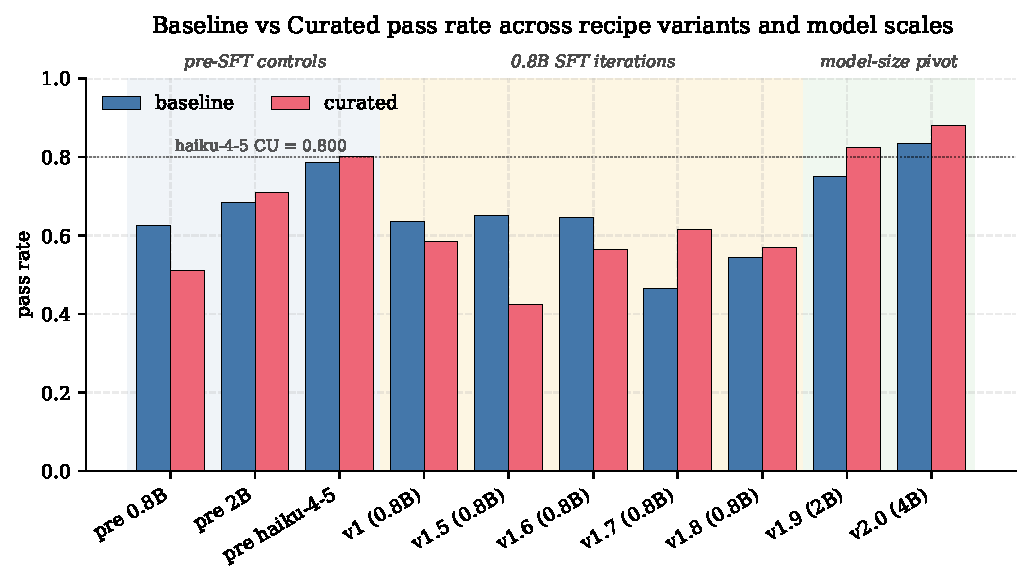
\includegraphics[width=\linewidth]{figures/fig1_progression.pdf}
\caption{Baseline (\BL) and curated (\CU) pass rates across all eleven evaluated configurations: pre-SFT controls, the five 0.8B SFT iterations, and the model-size pivot to 2B and 4B.}
\label{fig:progression}
\end{figure}

\begin{table}[h]
\centering
\small
\begin{tabularx}{\textwidth}{@{}l l Y r r r@{}}
\toprule
\textbf{Variant} & \textbf{Base} & \textbf{Recipe} & \textbf{BL} & \textbf{CU} & \textbf{$\Delta$} \\
\midrule
Pre-SFT 0.8B & 0.8B (HF)     & none & 0.625 & 0.510 & $-0.115$\,$\S$ \\
Pre-SFT 2B   & 2B (HF)       & none & 0.685 & 0.710 & $+0.025$ \\
Pre-SFT 4B   & 4B (HF)       & none & $0.000$\,$\dagger$ & $0.000$\,$\dagger$ & --- \\
Pre-SFT haiku-4-5 (ref) & claude-haiku-4-5 & none & 0.785 & 0.800 & $+0.015$ \\
\addlinespace
\textbf{v1}    & 0.8B & LoRA $r{=}8$, curated-only, 353 rows           & 0.635 & 0.585 & $-0.050$ \\
\textbf{v1.5}  & 0.8B & LoRA + BL+CU mixed corpus                       & 0.650 & 0.425 & $-0.225$ \\
\textbf{v1.6}  & 0.8B & LoRA + drop ceiling skills + chat-patch         & 0.645 & 0.565 & $-0.080$ \\
\textbf{v1.7}  & 0.8B & partial FT (top-6 layers + lm\_head)            & 0.465 & 0.615 & $+0.150$\,$\ddagger$ \\
\textbf{v1.8}  & 0.8B & partial FT + skill-block stripped from training & 0.545 & 0.570 & $+0.025$ \\
\textbf{v1.9}  & 2B   & LoRA $r{=}16$, curated-only, 353 rows           & \textbf{0.750} & \textbf{0.825} & $\boldsymbol{+0.075}$ \\
\textbf{v2.0}  & 4B   & LoRA $r{=}32$, curated-only, 353 rows           & \textbf{0.835} & \textbf{0.880} & $\boldsymbol{+0.045}$ \\
\bottomrule
\end{tabularx}
\caption{Recipe-by-recipe pass rates on the 200-task holdout, two conditions per task, single seed throughout, deterministic-mixed judge. All bases are Qwen3.5 dense models except where noted. All evaluations use HF transformers generation (matched path with the post-SFT students); the original Ollama-path pre-SFT 0.8B numbers ($0.510 / 0.565 / +0.055$) are documented in \S\ref{sec:path-mismatch} as historical. $\dagger$ Pre-SFT 4B's $0/0$ is a format-compliance artifact (\S\ref{sec:format-artifact}). $\ddagger$ v1.7's apparent $+\Delta$ is an artifact of \BL{} collapse, not differential learning (\S\ref{sec:v17-mode-collapse}). $\S$ Pre-SFT 0.8B HF matched-path: 334 deterministic-type episodes were re-scored locally via the deterministic extractor; the 33 \texttt{FREE\_FORM} tasks (66 episodes) carry their LLM-judged scores from the source \texttt{--force-llm-judge} run, which are valid for the deterministic-mixed dispatch (\S\ref{sec:path-mismatch}). LLM-only re-judge values (Table~\ref{tab:llm-only}) are systematically higher and reframe several of these results.}
\label{tab:headline}
\end{table}

\begin{table}[h]
\centering
\small
\begin{tabular}{@{}l r r r c c@{}}
\toprule
& \textbf{BL} & \textbf{CU} & \textbf{$\Delta$} & \textbf{McNemar $p$} & \textbf{bootstrap 95\% CI on $\Delta$} \\
\midrule
\textit{Pre-SFT base controls} \\
\textbf{pre-SFT 0.8B (HF)} & \textbf{0.665} & \textbf{0.590} & $\boldsymbol{-0.075}$ & --- & --- \\
pre-SFT 2B (HF)            & 0.755 & 0.815 & $+0.060$ & --- & --- \\
\textbf{pre-SFT 4B (HF)}   & \textbf{0.850} & \textbf{0.840} & $\boldsymbol{-0.010}$ & --- & --- \\
pre-SFT haiku-4-5 (ref)    & 0.955 & 0.985 & $+0.030$ & --- & --- \\
\addlinespace
\textit{Post-SFT students} \\
v1   (0.8B+LoRA)   & 0.710 & 0.705 & $-0.005$ & --- & --- \\
v1.9 (2B+LoRA)     & 0.815 & 0.915 & $+0.100$ & $0.0027$ & $[+0.040,\ +0.160]$ \\
v2.0 (4B+LoRA)     & 0.920 & 0.985 & $+0.065$ & $0.00098$ & $[+0.030,\ +0.105]$ \\
\bottomrule
\end{tabular}
\caption{LLM-only re-judge of all seven configurations under matched HF + LLM-only scoring (haiku via OAuth API, the rest via HF transformers): three pre-SFT base controls, three post-SFT students, one frontier reference. Removes the format-compliance gate (\S\ref{sec:format-artifact}) that biased the deterministic-mixed scoring in Table~\ref{tab:headline}. Three load-bearing observations: (i) v2.0 \CU{} ties the haiku reference at $0.985$ (197/200 identical pass count); (ii) pre-SFT base Δ is W-shaped --- $-0.075$ at 0.8B, $+0.060$ at 2B, $-0.010$ at 4B, $+0.030$ at haiku --- with two negative pockets at 0.8B and 4B; (iii) the SFT contribution to Δ-lift is roughly uniform across all three sizes ($+0.07$, $+0.04$, $+0.075$; Table~\ref{tab:sft-contribution}), so the variation in post-SFT Δ across sizes is dominated by the pre-SFT W-shape, not by SFT mechanism strength.}
\label{tab:llm-only}
\end{table}

\section{0.8B: Five Negative Results}

\subsection{v1: simplest recipe; deeper-than-it-looks SFT contribution under matched-path scoring}\label{sec:v1}
LoRA $r{=}8$/$\alpha{=}16$ on the 353-row \CU{} corpus for three epochs at $\mathrm{lr}{=}2{\times}10^{-4}$ lifts the 0.8B \BL{} pass-rate by $+1.0$\,pp ($0.625 \to 0.635$) and \CU{} by $+7.5$\,pp ($0.510 \to 0.585$) under the deterministic-mixed dispatch; $\Delta$ shifts from $-0.115$ (pre-SFT) to $-0.050$ (post-SFT), a $+0.065$ Δ-lift attributable to SFT. Earlier versions of this paper used a path-mismatched Ollama-path pre-SFT 0.8B baseline (Δ $+0.055$) and interpreted the post-SFT $\Delta -0.050$ as a ``Δ-flip'' diagnostic of ``format-only learning at 0.8B''; the procedural lift was characterised as absent and the 0.8B model as capacity-floored. Under the corrected Table~\ref{tab:headline} pre-SFT row (HF generation, matched path with v1; \S\ref{sec:path-mismatch}) the picture inverts: SFT delivers a clean $+0.065$ Δ-lift at 0.8B, comparable to the 2B and 4B SFT Δ-lifts.

\paragraph{Two scorings agree on direction.} Under matched-path LLM-only scoring (Table~\ref{tab:llm-only}), pre-SFT 0.8B lands at \BL{} $0.665$ / \CU{} $0.590$ / $\Delta -0.075$ and v1 lands at $0.710 / 0.705 / -0.005$, giving an SFT contribution of $+0.045$ \BL, $+0.115$ \CU, $+0.070$ Δ-lift. Under matched-path deterministic-mixed scoring (Table~\ref{tab:headline}), the SFT Δ-lift is $+0.065$. Both scorings agree the Δ-lift is positive and on the order of $+0.07$, comparable to the 4B SFT contribution ($+0.075$ Δ-lift) and larger than the 2B SFT contribution ($+0.040$ Δ-lift). What SFT does not do at 0.8B is push post-SFT Δ above zero, because base 0.8B sits in a deep procedure-hurts regime ($\Delta -0.115$ deterministic / $-0.075$ LLM-only) that SFT lifts to procedure-neutral, not to procedure-helps.

\paragraph{What survives of the original v1 diagnosis.} The absolute \CU{} pass rate at v1 ($0.585$ deterministic, $0.705$ LLM-only) does cluster with the v1.6 and v1.8 numbers in a $\sim$\,2\,pp band, and this cluster does not move with corpus composition or training-recipe variation (\S\ref{sec:0.8b-summary}). What clusters is the post-SFT \emph{absolute} pass rate, which is bounded by base 0.8B's reasoning capability; what does not cluster is the SFT-attributable Δ-lift, which is comparable to the 4B Δ-lift in matched-path comparison. The capacity-floor diagnosis was correct for absolute pass rate; it was wrong for the SFT mechanism's differential contribution.

\subsection{v1.5--v1.6: corpus composition does not unlock differential lift}
Adding baseline-passing rows to the SFT corpus (v1.5; teaching the model to produce procedural responses both with and without skill-block presence) collapses \CU{} pass-rate to $0.425$. Dropping ceiling-passing skills (v1.6; removing tasks where the base already passes $\geq\!0.90$ to avoid the model learning to add procedure overhead on tasks it can solve directly) lands at $0.645/0.565$ --- equivalent to v1 within noise.

\subsection{v1.7: full-rank partial FT and the mode-collapse artifact}\label{sec:v17-mode-collapse}
Replacing LoRA with full-rank fine-tuning of the top-6 layers + \texttt{lm\_head} + final \texttt{norm} (using 8-bit Adam to fit GPU budget) produces an apparent positive $\Delta$ ($+0.150$) but with \BL{} pass-rate \emph{collapsed} to $0.465$ --- substantially below the matched-path pre-SFT 0.8B \BL{} of $0.625$ (\S\ref{sec:path-mismatch}). Inspection of v1.7 \BL{} failures reveals the model emits ``\texttt{Step 1 (SKILL block: \dots)}'' prefaces and procedural step language even when no skill block is in the system prompt --- i.e.\ the model has learned to expect a skill block and hallucinates one when absent. The $+0.150$ $\Delta$ does not reflect the model learning to use skill blocks; it reflects the model losing the ability to function without one.

\subsection{v1.8: skill-block stripping fixes mode collapse, no new ceiling}
Stripping the skill block from the system prompt of every training row (so the model never sees a skill block during training, only the procedural response) recovers \BL{} ($0.545$) but lands \CU{} at $0.570$ --- within the $0.565$--$0.585$ cluster shared by v1, v1.6, and v1.8. The mode-collapse failure mode is fixed; no new ceiling is unlocked.

\subsection{0.8B summary}\label{sec:0.8b-summary}
Three well-formed variants (v1, v1.6, v1.8) cluster \CU{} within 2\,pp under deterministic judging (and within $\sim$\,1\,pp under LLM-only judging at v1, by re-judge). The cluster does not move with corpus composition, recipe, chat-template patches, or partial fine-tuning. \emph{The post-SFT absolute pass rate at 0.8B is bounded by base-model reasoning capability, regardless of recipe.} Note (per \S\ref{sec:v1}) that the 2B/4B-style ``SFT does no work at 0.8B'' interpretation is a path-mismatch artifact; under matched-path scoring, SFT's Δ-lift at 0.8B is $+0.070$, comparable to 4B. What the 0.8B negative results constrain is the absolute-pass-rate axis, not the SFT mechanism.

\section{2B and 4B: Model Size as the Decisive Axis}

\subsection{v1.9 (2B): SFT contribution is positive and outside binomial noise}\label{sec:v19}
Same recipe shape as v1 (LoRA, curated-only, 353 rows, 3 epochs), bumped to $r{=}16$/$\alpha{=}32$ to give the larger base more LoRA capacity, on \Qwent. Result: \BL{} $0.750$ / \CU{} $0.825$ / $\Delta$ $+0.075$ (paired-bootstrap 95\% CI $[+0.020, +0.130]$; McNemar $\chi^2{=}5.60$, $p{=}0.018$ on a single seed; \S\ref{sec:stats}).

A pre-SFT 2B control ($0.685/0.710$) attributes the lift over pre-SFT 0.8B (Table~\ref{tab:attribution}). On this measurement, the procedural-$\Delta$ lifts from $+0.025$ (pre-SFT) to $+0.075$ (post-SFT), a $+5$\,pp differential procedural-application lift attributable to SFT, and the absolute \CU{} contribution attributable to SFT is $+11.5$\,pp on top of base 2B's $0.710$. The corresponding 0.8B and 4B SFT contributions are documented in \S\ref{sec:v1} and \S\ref{sec:v20}; under matched-path LLM-only scoring all three SFT Δ-lifts cluster in a $4$\,pp band ($+0.040$ to $+0.075$, Table~\ref{tab:sft-contribution}).

\begin{figure}[h]
\centering
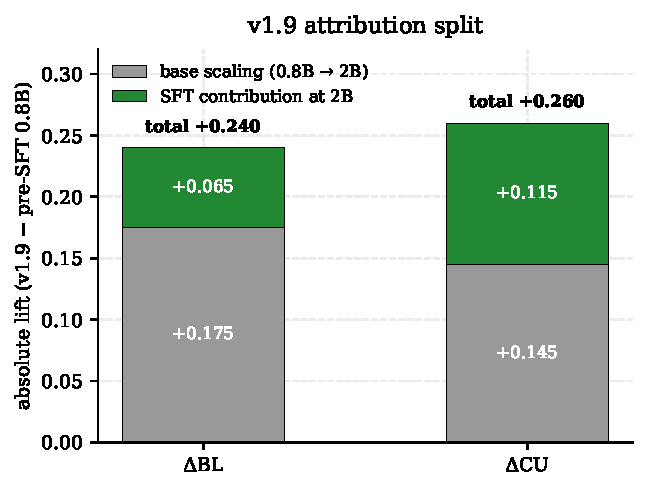
\includegraphics[width=0.5\linewidth]{figures/fig4_attribution.pdf}
\caption{v1.9 lift over pre-SFT 0.8B decomposed into base-model scaling (gray; measured between the two pre-SFT controls) and SFT contribution at 2B (green; the residual from pre-SFT 2B to v1.9). The SFT contribution is +6.5\,pp on \BL{} and +11.5\,pp on \CU.}
\label{fig:attribution}
\end{figure}

\begin{table}[h]
\centering
\small
\begin{tabular}{@{}l rr rr@{}}
\toprule
& \multicolumn{2}{c}{\textbf{deterministic-mixed}} & \multicolumn{2}{c}{\textbf{LLM-only (matched-path)}} \\
\cmidrule(lr){2-3} \cmidrule(lr){4-5}
& $\Delta$BL & $\Delta$CU & $\Delta$BL & $\Delta$CU \\
\midrule
Base scaling 0.8B $\to$ 2B  & $+0.060$ & $+0.200$ & $+0.090$ & $+0.225$ \\
SFT contribution at 2B      & $+0.065$ & $\mathbf{+0.115}$ & $+0.060$ & $\mathbf{+0.100}$ \\
\midrule
Total v1.9 vs pre-SFT 0.8B  & $+0.125$ & $+0.315$ & $+0.150$ & $+0.325$ \\
SFT $\Delta$-lift at 2B     & \multicolumn{2}{c}{$+0.025 \to +0.075$ ($\boldsymbol{+0.050}$)} & \multicolumn{2}{c}{$+0.060 \to +0.100$ ($\boldsymbol{+0.040}$)} \\
\bottomrule
\end{tabular}
\caption{v1.9 attribution split, under both judging paths. Both columns now use matched-path pre-SFT controls: deterministic-mixed uses pre-SFT 0.8B (HF, $0.625/0.510$; \S\ref{sec:path-mismatch}) and pre-SFT 2B (HF, $0.685/0.710$); LLM-only uses pre-SFT 0.8B (HF + LLM-only, $0.665/0.590$), pre-SFT 2B (HF + LLM-only, $0.755/0.815$), and v1.9 LLM-only ($0.815/0.915$). The SFT-attributable Δ-lift at 2B is $+0.050$ under deterministic-mixed and $+0.040$ under LLM-only --- consistent within $1$\,pp across both judging paths even as absolute magnitudes shift. The matched-path 0.8B and 4B SFT attribution splits are in Table~\ref{tab:sft-contribution}; SFT Δ-lift at 0.8B is $+0.065$ deterministic / $+0.070$ LLM-only, at 4B is $+0.075$ LLM-only.}
\label{tab:attribution}
\end{table}

\subsection{The Haiku-comparison observation, before and after format-tolerant re-judge}\label{sec:compute-efficiency}

A natural question is how SFT'd students compare against a frontier reference on this bench. We had originally framed this as a compute-efficiency observation: under the deterministic-mixed dispatch, the post-SFT 2B \CU{} pass-rate ($0.825$) exceeded the pre-SFT Claude Haiku 4.5 reference of $0.800$, while the pre-SFT 2B base ($0.710$) did not, suggesting the crossing was attributable to the 353-row SFT recipe.

Two findings in this paper undermine this framing and we present the corrected picture instead.

\textbf{The format-compliance artifact (\S\ref{sec:format-artifact}) penalised Haiku more than it penalised the SFT'd students.} Under the LLM-only re-judge (Table~\ref{tab:llm-only}, \S\ref{sec:llm-rejudge}) Haiku's \CU{} pass-rate rises from $0.800$ to $0.985$ --- a $+18.5$\,pp shift, the largest of any student in the experiment. Haiku's free-form-prose conclusions were disproportionately rejected by the deterministic \texttt{ANSWER:}-line extractor; under fair scoring Haiku is at the bench's effective ceiling. Under LLM-only judging, v1.9 \CU{} ($0.915$) does \emph{not} cross Haiku ($0.985$); v2.0 \CU{} ($0.985$) ties Haiku at the ceiling (197/200 identical pass count). The original ``2B+SFT crosses Haiku'' framing was an artifact of the format-compliance gate.

\textbf{What survives the remediation.} v2.0 (4B+SFT) reaches the bench's effective ceiling under fair scoring, matching the frontier reference. With pre-SFT 4B now measured at \CU{} $0.840$ under fair judging, we can rule out the strongest version of the deflationary alternative: the 4B base does \emph{not} already match Haiku before SFT, and the v2.0 ties Haiku precisely because SFT contributed $+0.145$ \CU{} on top of base 4B (\S\ref{sec:v20}). We still resist a sharp compute-efficiency claim because Haiku's parameter count is not published and community estimates span roughly $10^{10}$\,--\,$3{\times}10^{10}$ parameters with no anchor; Opus 4.7 wrote the corpus content, generated the SFT traces, and judged both students, so the comparison sits inside a structurally biased judging path (\S\ref{sec:threats}, partially closed by the cross-family validation in \S\ref{sec:cross-family}); and the SFT student is in-distribution for the bench while Haiku is being asked cold.

The honest summary is: under fair judging, v2.0 (4B+SFT) and Haiku are tied at the bench's curated ceiling on tasks of this construction style. With the pre-SFT 4B baseline now measured (\CU{} $0.840$), the SFT contribution at 4B is $+0.145$ \CU{} and the v2.0$=$Haiku comparison is attributable to that SFT contribution rather than to base scaling alone.

\subsection{v2.0 (4B): the SFT contribution at 4B is on par with the SFT contribution at 0.8B in differential terms}\label{sec:v20}

Same recipe at LoRA $r{=}32$/$\alpha{=}64$ on \Qwenf. Result: \BL{} $0.835$ / \CU{} $0.880$ / $\Delta$ $+0.045$ under deterministic judging (paired-bootstrap 95\% CI $[+0.005, +0.085]$; McNemar exact $p{=}0.049$ on a single seed); $0.985 / 0.920 / +0.065$ under LLM-only re-judge (CI $[+0.030, +0.105]$, McNemar exact $p{=}0.00098$). The LLM-only $\Delta$ comfortably survives Bonferroni correction across the two per-model tests in Table~\ref{tab:stats-per-model}; the deterministic-judge $p{=}0.049$ would not.

\paragraph{Pre-SFT 4B closes the attribution gap.} A fresh pre-SFT 4B evaluation under format-tolerant scoring lands at \BL{} $0.850$ / \CU{} $0.840$ / $\Delta$ $-0.010$. The procedure does \emph{not} help base 4B and mildly hurts it. Spot-checks of pre-SFT 4B responses confirm coherent step-by-step reasoning; the slightly negative Δ reflects that the 5-step procedure introduces sub-inference error opportunities on tasks the base can already one-shot, while curated responses sometimes follow the procedure into less-defensible conclusions on tasks the base would otherwise have answered directly.

\paragraph{The SFT contribution at 4B in differential terms.} Combining the v2.0 LLM-only result with pre-SFT 4B LLM-only:
\begin{itemize}[leftmargin=*, nosep]
    \item Absolute \BL{} contribution: $+0.070$ ($0.850 \to 0.920$)
    \item Absolute \CU{} contribution: $+0.145$ ($0.840 \to 0.985$)
    \item Procedural Δ-lift: $+0.075$ ($-0.010 \to +0.065$)
\end{itemize}
Compared across all three model sizes under matched-path LLM-only scoring (Table~\ref{tab:sft-contribution}), the 4B Δ-lift of $+0.075$ is on par with the 0.8B Δ-lift of $+0.070$ and larger than the 2B Δ-lift of $+0.040$. The absolute \CU{} contribution at 4B ($+0.145$) is the largest in the experiment, but the differential Δ-lift is not uniquely large at 4B; the SFT mechanism delivers roughly capacity-invariant Δ-lift (range $+0.040$ to $+0.075$, all three sizes) within a $4$\,pp band.

\begin{table}[h]
\centering
\small
\begin{tabular}{@{}l rrr rrr@{}}
\toprule
& \multicolumn{3}{c}{\textbf{Pre-SFT base (LLM-only)}} & \multicolumn{3}{c}{\textbf{SFT contribution}} \\
\cmidrule(lr){2-4} \cmidrule(lr){5-7}
& BL & CU & $\Delta$ & $\Delta$BL & $\Delta$CU & $\Delta$-lift \\
\midrule
0.8B (v1)   & 0.665 & 0.590 & $-0.075$ & $+0.045$ & $+0.115$ & $\boldsymbol{+0.070}$ \\
2B (v1.9)   & 0.755 & 0.815 & $+0.060$ & $+0.060$ & $+0.100$ & $\boldsymbol{+0.040}$ \\
4B (v2.0)   & 0.850 & 0.840 & $-0.010$ & $+0.070$ & $+0.145$ & $\boldsymbol{+0.075}$ \\
\bottomrule
\end{tabular}
\caption{SFT contribution across all three model sizes under matched HF + LLM-only scoring. The Δ-lift attributable to SFT is in a tight $4$\,pp band ($+0.040$ to $+0.075$) across an order-of-magnitude in base-model capacity; the absolute \CU{} contribution is in a similar band ($+0.100$ to $+0.145$). The variation in post-SFT Δ across sizes is dominated by the pre-SFT base trajectory, which is W-shaped (negative at 0.8B and 4B, positive at 2B and frontier-class haiku-4-5; cf.\ Table~\ref{tab:llm-only}).}
\label{tab:sft-contribution}
\end{table}

\paragraph{The bench saturation diagnosis splits in two.} The v1.9$\to$v2.0 \emph{post-SFT} Δ shrinkage ($+0.100 \to +0.065$ under LLM-only) is directionally consistent with bench saturation but not statistically distinguishable from sampling noise on the v1.9-vs-v2.0 adjacent-pair test (\S\ref{sec:stats}). The previous version of this paper used that shrinkage to argue ``saturation = SFT contribution shrinks''; with pre-SFT 4B in hand, this is falsified for the SFT contribution. The remaining accurate version of the saturation claim is narrower: the absolute pass rate is saturated (v2.0 \CU{} ties Haiku at $0.985$); the SFT mechanism is not (Δ-lift roughly uniform across all three sizes). What changes across the post-SFT trajectory is the pre-SFT starting point, not the SFT mechanism's strength. Two separate things were being conflated under one ``saturation'' label.

\paragraph{Why does pre-SFT base Δ trace a W-shape?} The pre-SFT trajectory of base-model procedural responsiveness is non-monotone with two negative pockets: $-0.075$ at 0.8B, $+0.060$ at 2B, $-0.010$ at 4B, $+0.030$ at frontier-class haiku. Two distinct mechanisms plausibly contribute: (a) very small bases (0.8B) lack the capacity to follow the procedure correctly --- the 5-step structure introduces sub-inference errors at every step, and the base cannot recover from them, so the procedure compounds errors rather than scaffolding correct reasoning; (b) competent-but-not-frontier bases (4B) are capable enough to solve baseline tasks directly but not capable enough to use the procedure productively --- the procedure adds overhead without adding signal. The two intermediate (2B) and frontier (haiku) regimes both have positive Δ for different reasons: 2B is in a sweet spot where the procedure scaffolds reasoning the base would otherwise skip; haiku has the native capacity to use the procedure as intended. SFT's distinctive value is uniform across both negative-Δ pockets: it lifts Δ by $+0.07$ at both 0.8B and 4B, sufficient to get 0.8B to procedure-neutral and 4B into procedure-helps territory.

\paragraph{Per-skill structure.} Figure~\ref{fig:per-skill} shows the v2.0 procedural-$\Delta$ broken down by skill (deterministic-judge counts). Eleven skills lift on \CU{} (concentrated on interpretive and spatial-social skills); 25 are flat (mostly because \BL{} is at ceiling); 4 regress under deterministic judging (deductive-logic skills where the base has ceiling competence and the 5-step procedure introduces sub-inference error opportunities). Under LLM-only judging the regression cluster shrinks to one skill, consistent with the curated-condition deterministic-judge bias documented in \S\ref{sec:llm-rejudge}.

\paragraph{Per-skill BL-vs-Δ correlation: regime-asymmetric story holds at the skill level (qualitatively).} Figure~\ref{fig:per-skill-bl-vs-delta} plots per-skill Δ against per-skill baseline pass rate at v2.0 under LLM-only judging. Spearman $\rho(\BL, \Delta) = -0.227$ across $n{=}40$ skills (two-sided $p \approx 0.15$, not significant at conventional thresholds; the analysis is underpowered because 29/40 skills are tied at \BL{} $= 1.0$, collapsing to the same rank). On the non-ceiling subset (skills with $\BL < 1.0$, $n{=}11$), the correlation strengthens to $\rho = -0.455$ ($p \approx 0.13$); the negative slope is qualitatively consistent in both subsets but neither reaches conventional significance at this $n$. The lift cluster has mean baseline $0.709$; the flat cluster has mean baseline $1.000$. We treat this as qualitative evidence rather than a load-bearing statistical claim, consistent with Figure~\ref{fig:per-skill-bl-vs-delta}'s caption hedge: the procedure helps where the base struggles and is silent where the base is at ceiling, and the negative slope is the per-skill miniature of the cross-scale regime-asymmetric finding (\S\ref{sec:what-sft-taught}).

\begin{figure}[h]
\centering
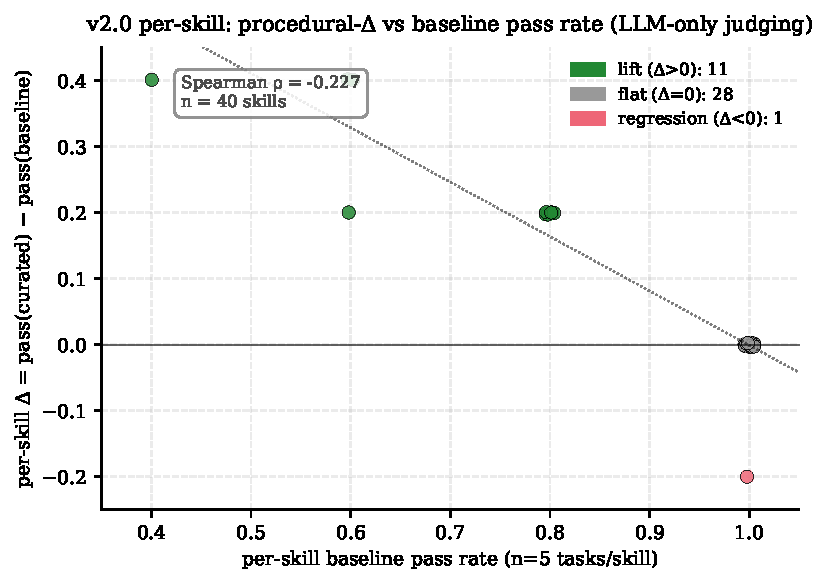
\includegraphics[width=0.78\linewidth]{figures/fig5_per_skill_bl_vs_delta.pdf}
\caption{Per-skill procedural-Δ at v2.0 versus per-skill baseline pass rate (LLM-only judging, $n{=}5$ tasks per skill, 40 skills). Spearman $\rho = -0.227$. Skills where the base is already at ceiling on baseline cannot benefit from procedure injection (flat cluster, BL $\approx 1.0$); skills with lower baseline have the most Δ headroom (lift cluster, mean BL $\approx 0.71$). One regression-cluster skill (\texttt{equivocation}) has BL $1.0$ and CU $0.8$, fitting the same pattern: the procedure adds friction on a skill the base could already one-shot. The negative slope is qualitative evidence that SFT's distinctive value is in scaffolding skills the base struggles with, not in lifting already-saturated skills.}
\label{fig:per-skill-bl-vs-delta}
\end{figure}

\begin{figure}[h]
\centering
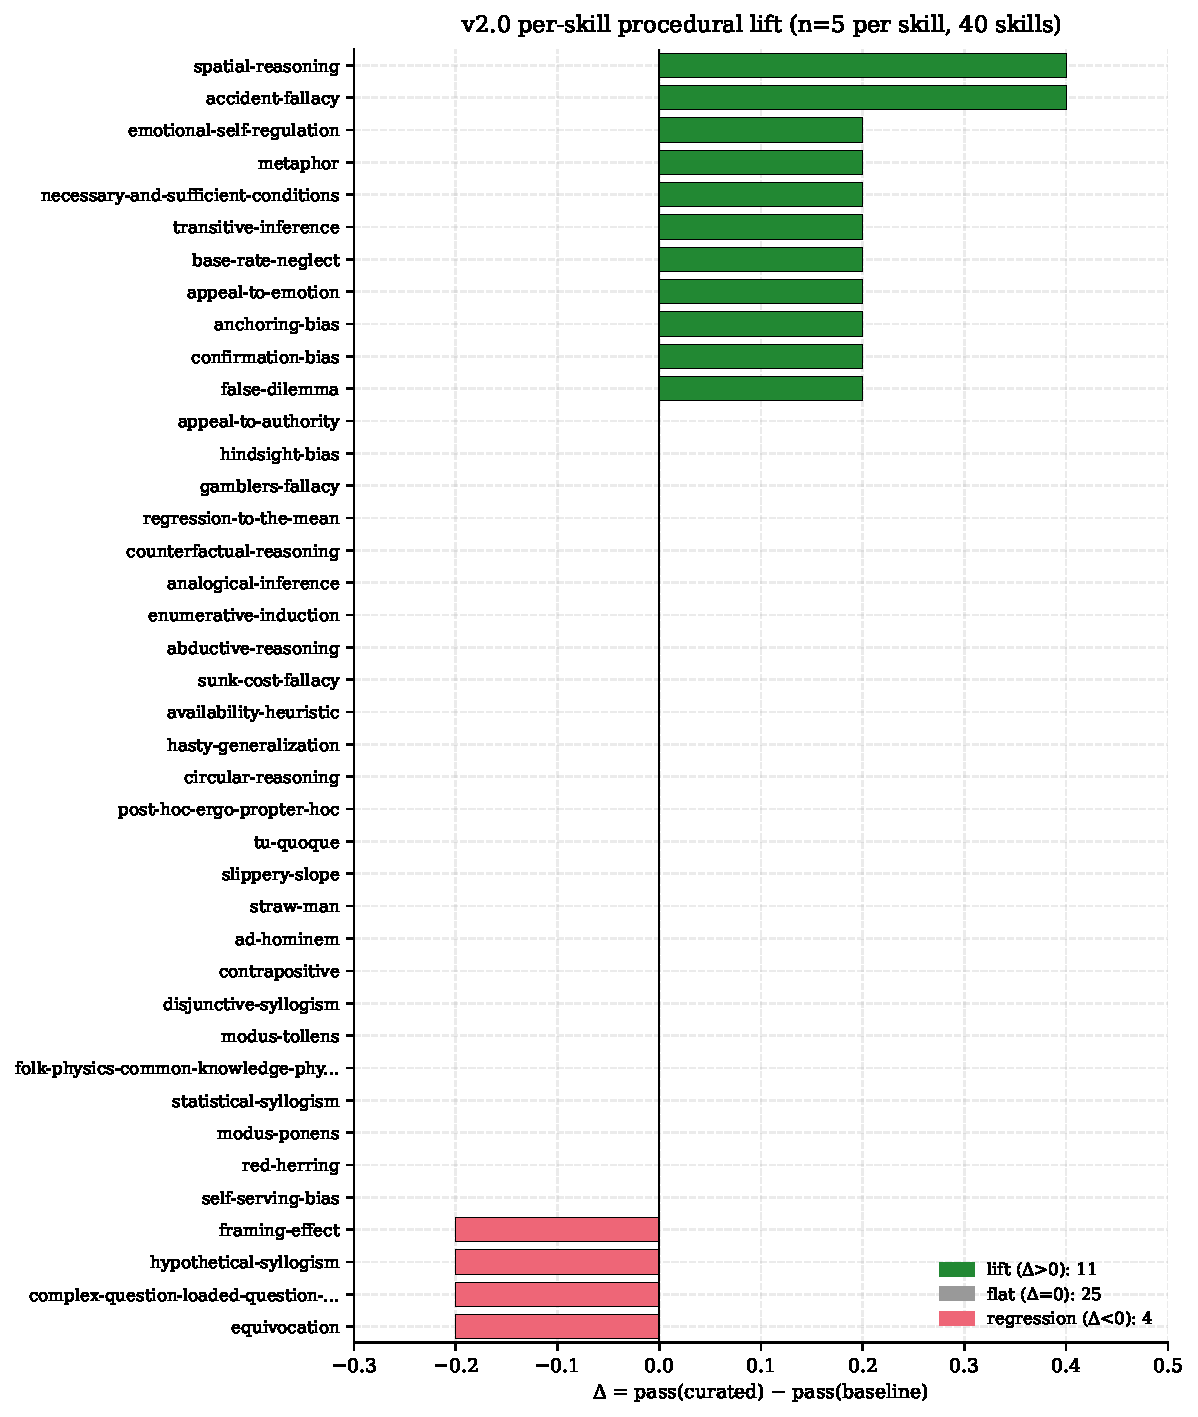
\includegraphics[width=0.85\linewidth]{figures/fig2_per_skill_v2_0.pdf}
\caption{Per-skill procedural-$\Delta$ at v2.0 ($n{=}5$ per skill, 40 skills). 11 skills lift on \CU; 25 are flat (mostly because \BL{} is already at ceiling); 4 regress. The lift cluster concentrates on interpretive and spatial-social skills; the regression cluster on deductive-logic skills where the model has ceiling competence on \BL.}
\label{fig:per-skill}
\end{figure}

\subsection{Statistical tests of the per-model and cross-model $\Delta$ estimates}\label{sec:stats}

Each task is run in both \BL{} and \CU{} conditions, so the verdicts are paired. We run McNemar's test (continuity-corrected $\chi^2$ for $n_{\mathrm{discordant}} \geq 25$, exact binomial otherwise) per model, and a paired bootstrap (10{,}000 resamples of \texttt{task\_uid} with replacement) for 95\% CIs on $\Delta$. Cross-model: we resample v1.9 and v2.0 independently and report a one-sided bootstrap test for $H_0\!: \Delta_{\mathrm{v1.9}} \leq \Delta_{\mathrm{v2.0}}$ (the direction predicted by the saturation hypothesis). All tests are on a single seed per condition.

\begin{table}[h]
\centering
\small
\begin{tabular}{@{}l c c c c@{}}
\toprule
& \multicolumn{2}{c}{\textbf{deterministic-mixed}} & \multicolumn{2}{c}{\textbf{LLM-only re-judge}} \\
\cmidrule(lr){2-3}\cmidrule(lr){4-5}
& $\Delta$ & McNemar $p$ / 95\% CI & $\Delta$ & McNemar $p$ / 95\% CI \\
\midrule
v1.9 & $+0.075$ & $\chi^2{=}5.60$, $p{=}0.018$ & $+0.100$ & $\chi^2{=}9.03$, $p{=}0.0027$ \\
     &          & CI $[+0.020,\ +0.130]$       &          & CI $[+0.040,\ +0.160]$ \\
v2.0 & $+0.045$ & exact, $p{=}0.049$           & $+0.065$ & exact, $p{=}0.00098$ \\
     &          & CI $[+0.005,\ +0.085]$       &          & CI $[+0.030,\ +0.105]$ \\
\bottomrule
\end{tabular}
\caption{Per-model paired tests on the procedural-$\Delta$, under both judging paths. Both models have a positive $\Delta$ with bootstrap CI excluding zero in both paths. Under LLM-only re-judge, v2.0's $p{=}0.00098$ comfortably survives Bonferroni correction across the two tests (the deterministic-mixed $p{=}0.049$ would not). Neither test is replicated across seeds.}
\label{tab:stats-per-model}
\end{table}

For the cross-model saturation test, the result is essentially unchanged across judging paths:
\begin{itemize}[leftmargin=*,nosep]
  \item Deterministic-mixed: $\Delta_{\mathrm{v1.9}} - \Delta_{\mathrm{v2.0}} = +0.030$, CI $[-0.040,\ +0.100]$, one-sided $p = 0.225$.
  \item LLM-only re-judge: $\Delta_{\mathrm{v1.9}} - \Delta_{\mathrm{v2.0}} = +0.035$, CI $[-0.040,\ +0.105]$, one-sided $p = 0.191$.
\end{itemize}

The CI includes zero in both paths. The $\Delta$-shrinkage from v1.9 to v2.0 is consistent with bench saturation in direction but is \emph{not statistically distinguishable from sampling noise at the present sample size}, regardless of judging path. The cross-student 4-point trajectory in \S\ref{sec:llm-rejudge} is more informative than this adjacent-pair test, since it constrains $\Delta$ across a 4-point capability range rather than at a single pair. Confirming the saturation pattern with adjacent-pair statistics would require either (a) larger $n$ ($\sim\!800$--$1200$ per condition for $80\%$ power to detect an effect of this magnitude), (b) a bench where the procedural lift is 2--3$\times$ larger so the absolute $\Delta$ is more robustly measurable, or (c) multi-seed evaluation to reduce per-condition variance.

\begin{figure}[h]
\centering
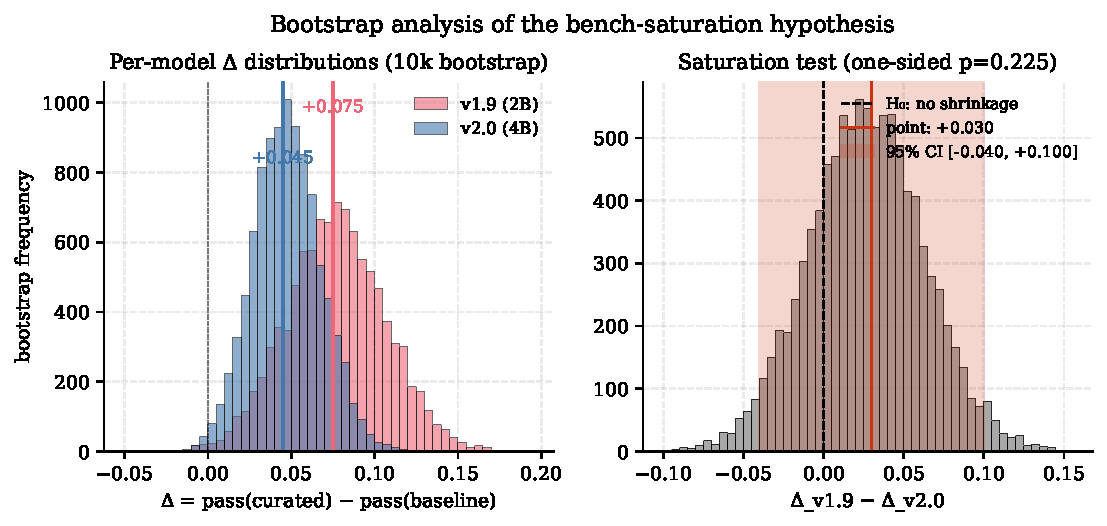
\includegraphics[width=\linewidth]{figures/fig3_bootstrap.pdf}
\caption{Left: bootstrap distributions of the procedural-$\Delta$ for v1.9 and v2.0 (10{,}000 resamples of paired \texttt{task\_uid}s). Both distributions sit above zero (the dashed line) but overlap substantially. Right: distribution of the difference $\Delta_{\mathrm{v1.9}} - \Delta_{\mathrm{v2.0}}$. The 95\% CI shaded in red includes zero, and the one-sided test for the saturation hypothesis returns $p{=}0.225$. Direction is consistent with saturation; magnitude is not statistically distinguishable from noise.}
\label{fig:bootstrap}
\end{figure}

\subsection{LLM-only re-judge: closing the format gap}\label{sec:llm-rejudge}

The format-compliance artifact documented in \S\ref{sec:format-artifact} blocks clean attribution at 4B and constrains the interpretation of the deterministic-judge headline numbers. The natural remediation is to re-route every episode through the LLM judge regardless of its task type, since the LLM judge already accepts free-form conclusions on \texttt{FREE\_FORM} tasks. We applied this remediation to all seven available configurations (v1, v1.9, v2.0, haiku-4-5, pre-SFT 0.8B, pre-SFT 2B, pre-SFT 4B); for the post-SFT students and haiku we re-ran the judge over the existing model responses (no model regeneration), and for the pre-SFT base models we ran fresh HF-transformers evaluations with \texttt{--force-llm-judge} to bypass the deterministic dispatch. Numbers are in Table~\ref{tab:llm-only}; the SFT-contribution decomposition under matched scoring is in Table~\ref{tab:sft-contribution}.

\paragraph{All pass rates rise; haiku rises the most.} The deterministic-mixed judge under-counted passes universally (Table~\ref{tab:rejudge-deltas}). Even the SFT'd students, which were trained to produce \texttt{ANSWER:} format, occasionally emitted alternative phrasings (``Final Answer: X'', ``I conclude X'', or stating the answer in prose) that the deterministic extractor missed. Haiku, which was never trained on the bench's response format, was penalised the most --- $+17$\,pp on \BL{} and $+18.5$\,pp on \CU{} relative to the deterministic-mixed scoring. This is the cleanest direct evidence that the format-compliance gate biased the bench against students whose response style does not match the SFT distribution.

\begin{table}[h]
\centering
\small
\begin{tabular}{@{}l r r r@{}}
\toprule
& $\Delta$BL & $\Delta$CU & $\Delta\Delta$ \\
\midrule
v1   (0.8B+LoRA)   & $+0.075$ & $+0.120$ & $+0.045$ \\
v1.9 (2B+LoRA)     & $+0.065$ & $+0.090$ & $+0.025$ \\
v2.0 (4B+LoRA)     & $+0.085$ & $+0.105$ & $+0.020$ \\
haiku-4-5 (ref)    & $+0.170$ & $+0.185$ & $+0.015$ \\
\bottomrule
\end{tabular}
\caption{Score shifts from deterministic-mixed (Table~\ref{tab:headline}) to LLM-only re-judge (Table~\ref{tab:llm-only}). All four students gain on both conditions; haiku gains the most. For the three SFT'd students, $\Delta$CU $>$ $\Delta$BL, meaning the deterministic judge was systematically biased \emph{against} the curated condition --- procedure-following responses bury conclusions in narration more often than direct-thinking responses do.}
\label{tab:rejudge-deltas}
\end{table}

\paragraph{The deterministic judge was biased against the curated condition.} For all three SFT'd students, $\Delta$CU exceeds $\Delta$BL by $2$--$4.5$\,pp under re-judge. When the procedure block is present, the model occasionally embeds its conclusion inside procedural narration (``\dots therefore the conclusion follows: X'') rather than ending with a literal \texttt{ANSWER: X} line. The deterministic judge under-counted curated wins systematically, under-stating the SFT contribution. The corrected $\Delta$ values in Table~\ref{tab:llm-only} are the more accurate measurement of the SFT-attributable differential procedural lift.

\paragraph{v1's negative $\Delta$ has a smaller absolute magnitude under fair scoring.} Under the deterministic dispatch, v1 has \CU{} below \BL{} ($\Delta = -0.050$); under LLM-only judging it tightens to $-0.005$ (essentially zero). Both are real measurements; the LLM-only number is the better one because it bypasses the format-compliance gate that under-counts curated wins (\S\ref{sec:format-artifact}). Crucially, both judging paths agree the SFT Δ-lift at 0.8B is positive: $+0.065$ deterministic-mixed (matched-path Table~\ref{tab:headline}; \S\ref{sec:path-mismatch}) and $+0.070$ LLM-only --- consistent within $5$\,pp. SFT lifts pre-SFT 0.8B from a deep procedure-hurts regime ($\Delta -0.115$ deterministic / $-0.075$ LLM-only) to procedure-neutral ($\Delta -0.050$ / $-0.005$); what it does not do at 0.8B is push post-SFT Δ above zero, because the absolute pass-rate ceiling at 0.8B is base-capacity-bounded.

\paragraph{Cross-student post-SFT trajectory under fair judging.} The four post-SFT LLM-only $\Delta$ values trace a single-peaked (rises then falls) trajectory across capability tier:
\begin{itemize}[leftmargin=*, nosep]
  \item v1   (0.8B + LoRA): $\Delta = -0.005$
  \item v1.9 (2B  + LoRA, peak post-SFT $\Delta$): $\Delta = +0.100$
  \item v2.0 (4B  + LoRA): $\Delta = +0.065$
  \item haiku-4-5 (frontier reference, no SFT): $\Delta = +0.030$
\end{itemize}

\paragraph{Cross-student pre-SFT trajectory: W-shaped, with negative pockets at 0.8B and 4B.} Under matched HF + LLM-only scoring, the pre-SFT base trajectory is non-monotone with two negative-Δ pockets:
\begin{itemize}[leftmargin=*, nosep]
  \item \textbf{pre-SFT 0.8B (HF, LLM-only): $\Delta = -0.075$ --- deepest trough}
  \item pre-SFT 2B (HF, LLM-only): $\Delta = +0.060$
  \item \textbf{pre-SFT 4B (HF, LLM-only): $\Delta = -0.010$ --- shallow trough}
  \item pre-SFT haiku-4-5 (LLM-only): $\Delta = +0.030$
\end{itemize}
Both 0.8B and 4B are in regimes where the procedure injection actively hurts the base; 2B and haiku are in regimes where it helps. The 0.8B and 4B troughs likely reflect different mechanisms: at 0.8B the base lacks the capacity to follow the 5-step procedure correctly (errors compound at every step), while at 4B the base is competent enough to solve baseline tasks directly so the procedure adds overhead without adding signal. (See \S\ref{sec:v20} for fuller mechanism discussion.)

\paragraph{The SFT-attributable Δ-lift is roughly capacity-invariant.} Combining the pre-SFT and post-SFT trajectories under matched scoring (Table~\ref{tab:sft-contribution}):
\begin{itemize}[leftmargin=*, nosep]
    \item 0.8B (v1 vs pre-SFT 0.8B HF): pre-SFT $\Delta -0.075 \to$ post-SFT $\Delta -0.005$, SFT Δ-lift $\boldsymbol{+0.070}$
    \item 2B (v1.9 vs pre-SFT 2B): pre-SFT $\Delta +0.060 \to$ post-SFT $\Delta +0.100$, SFT Δ-lift $\boldsymbol{+0.040}$
    \item 4B (v2.0 vs pre-SFT 4B): pre-SFT $\Delta -0.010 \to$ post-SFT $\Delta +0.065$, SFT Δ-lift $\boldsymbol{+0.075}$
\end{itemize}
The SFT contribution to the differential procedural lift sits in a tight $4$\,pp band ($+0.040$ to $+0.075$) across an order of magnitude in base-model capacity. Two earlier framings of this work were path-mismatch artifacts:
\begin{enumerate}[leftmargin=*, nosep]
  \item v1's ``format-only learning at 0.8B'' was based on comparing v1 deterministic $\Delta = -0.050$ against pre-SFT 0.8B Ollama deterministic $\Delta = +0.055$ (both deterministic-mixed), suggesting the SFT had reversed Δ at 0.8B. Under matched-path HF scoring, v1's SFT Δ-lift is $+0.065$ (det-mixed) or $+0.070$ (LLM-only), both positive and on par with 4B. The earlier diagnosis confused the absolute-pass-rate ceiling at 0.8B (which is base-capacity-bound) with the SFT mechanism (which delivers comparable Δ-lift at 0.8B as at 4B).
  \item The previous version of this paper used the post-SFT $\Delta$-shrinkage (v1.9 $+0.100 \to$ v2.0 $+0.065$) to argue ``SFT contribution amplifies with capacity at 4B.'' With matched-scoring pre-SFT 0.8B in hand, the 4B Δ-lift of $+0.075$ is on par with 0.8B's $+0.070$, not uniquely large. The accurate framing is mechanism-uniformity rather than capacity-conditional amplification.
\end{enumerate}
What changes across the post-SFT trajectory is the pre-SFT starting point (W-shape: $-0.075, +0.060, -0.010, +0.030$), not the SFT mechanism's strength.

\paragraph{What this remediation does not address.} It removes the format-compliance gate as a confound for all seven students whose responses we have under fair judging. It does not address (a) judge-overlap with corpus generation (addressed separately in \S\ref{sec:cross-family}), or (b) single-seed variance.

\subsection{Cross-family judge cross-validation: GPT-5.4 vs Opus 4.7}\label{sec:cross-family}

The judge-overlap concern (\S\ref{sec:threats}) was the strongest unbounded methodological concern in the experiment: Opus 4.7 wrote the procedural skill catalog, synthesized the tasks, generated the SFT-corpus traces, and judged both pre-SFT and post-SFT responses. The concern: the judge may favor responses that resemble Opus's own style. To bound the magnitude, we ran a non-Anthropic-family second judge (GPT-5.4 via OpenRouter) on the LLM-only re-judge episodes for all seven configurations.

\begin{table}[h]
\centering
\small
\begin{tabular}{@{}l c c c c c@{}}
\toprule
& \multicolumn{2}{c}{\textbf{Opus 4.7 LLM-only}} & \multicolumn{2}{c}{\textbf{GPT-5.4 (OpenRouter)}} & \\
\cmidrule(lr){2-3}\cmidrule(lr){4-5}
& BL / CU & $\Delta$ & BL / CU & $\Delta$ & $\Delta$ shift \\
\midrule
v1   (0.8B+LoRA)        & 0.710 / 0.705 & $-0.005$ & 0.700 / 0.700 & $\;0.000$ & $+0.005$ \\
v1.9 (2B+LoRA)          & 0.815 / 0.915 & $+0.100$ & 0.815 / 0.915 & $+0.100$ & $\;0.000$ \\
v2.0 (4B+LoRA)          & 0.920 / 0.985 & $+0.065$ & 0.920 / 0.980 & $+0.060$ & $-0.005$ \\
haiku-4-5 (ref)         & 0.955 / 0.985 & $+0.030$ & 0.955 / 0.975 & $+0.020$ & $-0.010$ \\
\textbf{pre-SFT 0.8B}   & \textbf{0.665 / 0.590} & $\boldsymbol{-0.075}$ & \textbf{0.670 / 0.585} & $\boldsymbol{-0.085}$ & $-0.010$ \\
pre-SFT 2B              & 0.755 / 0.815 & $+0.060$ & 0.750 / 0.835 & $+0.085$ & $+0.025$ \\
\textbf{pre-SFT 4B}     & \textbf{0.850 / 0.840} & $\boldsymbol{-0.010}$ & \textbf{0.850 / 0.805} & $\boldsymbol{-0.045}$ & $\boldsymbol{-0.035}$ \\
\bottomrule
\end{tabular}
\caption{Cross-family judge cross-validation across all seven configurations / 2800 paired episodes. Per-episode agreement ranges from $93.25\%$ (pre-SFT 4B, 373/400) to $100.00\%$ (v1.9, 400/400, identical pass/fail verdicts on every episode). Cohen's $\kappa$ ranges from $0.754$ (pre-SFT 4B) to $1.000$ (v1.9). Pre-SFT 0.8B HF agreement is $98.50\%$ ($\kappa{=}0.968$). Headline $\Delta$ shifts $\leq 0.035$\,pp on every dataset; both judges agree on the direction of every per-student finding, including the W-shape's two negative-Δ pockets at 0.8B and 4B that drive the matched-path SFT attribution (\S\ref{sec:v20}).}
\label{tab:cross-family}
\end{table}

\paragraph{Agreement and the load-bearing finding.} The agreement is essentially perfect for the SFT'd students (v1.9: 400/400 identical verdicts; v2.0: 399/400; v1: 395/400). It is lowest on pre-SFT 4B (373/400, $\kappa=0.754$), the dataset where the base model produces the most genuinely-borderline responses. Crucially, the direction of every per-student finding is preserved across both judges. Both negative-Δ pockets in the W-shape are judge-invariant: pre-SFT 0.8B has Δ $\leq -0.075$ (Opus $-0.075$, GPT $-0.085$), and pre-SFT 4B has Δ $\leq 0$ (Opus $-0.010$, GPT $-0.045$). The SFT contribution at all three sizes is positive under both judges: Δ-lift $+0.070$ / $+0.085$ at 0.8B, $+0.040$ / $+0.015$ at 2B, $+0.075$ / $+0.105$ at 4B (Opus / GPT respectively).

\paragraph{Bound on the headline.} Across $2800$ paired episodes, the maximum headline-Δ shift between judges is $0.035$\,pp (pre-SFT 4B); the minimum agreement is $93.25\%$; the minimum $\kappa$ is $0.754$. Under a non-Anthropic-family second judge on non-Anthropic infrastructure, no headline conclusion changes direction across all seven cross-family-validated configurations. Cross-family bounds on the SFT contribution: at 0.8B, Δ-lift $[+0.070, +0.085]$; at 2B, Δ-lift $[+0.015, +0.040]$ (GPT credits base 2B with more procedural responsiveness than Opus does, narrowing the SFT-attributable component); at 4B, Δ-lift $[+0.075, +0.105]$. All three SFT contributions are positive under both judges. On every result, the direction is judge-invariant; only the magnitude varies, and only within tight bounds.

\paragraph{What cross-family validation does not close.} The cross-family judge bounds the \emph{judging-stage} judge-overlap concern. It does not address (a) corpus-generation overlap (Opus wrote the procedural rewrites, synthesized the tasks, generated the SFT-corpus traces; this is structurally unbounded by judging-stage cross-validation), (b) single-seed evaluation variance, or (c) cross-third-family judging (a Gemini or Llama judge would extend the bound). The judging-stage bound is itself substantial: the strongest single-axis methodological concern in the paper is now bounded quantitatively.

\subsection{Generality probe: v2.0 preserves out-of-distribution behavior}
We probe v1.9, v2.0, base 2B, and base 4B with a 52-prompt OOD battery (10 generality + 42 factual including 8 false-premise ``trick'' prompts) under a generic system prompt (not the \textsc{solver} prompt; Table~\ref{tab:generality}). The probe is a convenience sample, not a calibrated benchmark; we treat it as qualitative evidence of OOD behavior, not as a quantitative claim.

\begin{table}[h]
\centering
\small
\begin{tabular}{@{}lcccc@{}}
\toprule
& format-locked & factual HIT & trick CONFAB (eyeballed) & phantom skill block \\
\midrule
v1.9 (2B) & $0/52$ & $33/34$\,$\dagger$ & $6/8$ & $0/52$ \\
base 4B   & $0/52$ & $34/34$ & $\sim\!1/8$ & $0/52$ \\
v2.0 (4B) & $0/52$ & $34/34$ & $\mathbf{0/8}$ & $0/52$ \\
\bottomrule
\end{tabular}
\caption{Generality probe under generic system prompt. $\dagger$ v1.9 swapped \emph{Brave New World} attribution from Aldous Huxley to H.\,G.\,Wells --- a plausible-author confabulation absent from base 4B and v2.0.}
\label{tab:generality}
\end{table}

v1.9 introduced a small calibration regression on adversarial prompts: the SFT-induced ``produce a confident step-by-step answer'' prior leaks into out-of-distribution behavior, making v1.9 commit to plausible-sounding inventions where base 2B would refuse. v2.0 does not exhibit this --- the 4B base has enough native capacity to recognize false premises and refuse cleanly without the SFT shape overriding refusal.

The bench-time finding that 17.5\% of v2.0's \BL{} responses reference a ``skill block'' not present in the system prompt does \emph{not} extend to general-chat distributions: under a generic system prompt, the SFT-induced skill-block reflex is dormant ($0/52$). The phantom-mention is contextual to SFT-distribution-similar prompts.

\section{A Bench Format-Compliance Artifact}\label{sec:format-artifact}

The pre-SFT 4B attribution failure surfaces a property of the bench that is invisible when only SFT-trained students are evaluated: 88.5\% of the holdout uses a deterministic \texttt{ANSWER:}-line extractor, which heavily penalizes models that reason correctly but emit free-form conclusions. Base \Qwenf{} is such a model. Spot-checks of pre-SFT 4B responses on bench tasks confirm step-by-step reasoning that reaches the correct answer; the model simply does not consistently end with \texttt{ANSWER: <X>}, so the deterministic dispatch returns failure. The bench's $0/200$ for pre-SFT 4B should be read as ``format-compliance baseline $\approx 0$'', not ``reasoning $\approx 0$''.

This is a property of the present bench, but the issue generalises. Any post-SFT lift measured against a format-strict deterministic judge conflates three contributions: format learning (the model now emits the required line), format-conditional reasoning gating (the model reasons more reliably when constrained to a structured response), and procedural application (the model uses the injected skill). Without a base-model control evaluated under format-tolerant scoring, these are not separable. Plausible remedies for follow-up work include (a) a stricter base-model evaluation prompt that reliably hits the format target, (b) a format-tolerant judge for base controls (e.g.\ extracting the answer with an LLM call rather than a regex), or (c) restricting evaluation to \texttt{FREE\_FORM} tasks where an LLM judge is already in the loop.

In \S\ref{sec:llm-rejudge} we apply remediation (b) to all seven available configurations: re-running the LLM judge over the existing model responses for the SFT'd students and haiku, and running fresh HF evaluations under \texttt{--force-llm-judge} for the three pre-SFT base models (0.8B, 2B, 4B). Table~\ref{tab:llm-only} reports the resulting numbers. The remediation: (i) closes the v2.0 attribution gap (\S\ref{sec:v20}); (ii) yields the counter-intuitive finding that pre-SFT 4B has $\Delta \leq 0$ under both judging families; (iii) reveals that pre-SFT 0.8B HF/LLM-only has $\Delta = -0.075$, the deepest negative-Δ point in the trajectory, and that the v1 SFT contribution at 0.8B (Δ-lift $+0.070$) is comparable to 4B's --- falsifying the earlier ``format-only learning at 0.8B'' diagnosis (\S\ref{sec:v1}).

\section{Discussion}

\subsection{What did SFT actually teach?}\label{sec:what-sft-taught}
Across all three model sizes under matched-path scoring (Table~\ref{tab:sft-contribution}), SFT contributes a procedural Δ-lift in the $+0.040$ to $+0.075$ band on top of the pre-SFT base. Taking 2B as a representative case: $+11.5$\,pp absolute \CU{} pass-rate on top of base 2B's $0.710$, a $+6.5$\,pp lift on \BL{}, and a $+5$\,pp differential procedural-application lift ($\Delta$ from $+0.025$ to $+0.075$ deterministic, $+0.060$ to $+0.100$ LLM-only). The differential component is what distinguishes ``the model uses the injected procedure'' from ``the model just imitates the response shape''; pure format-learning would lift \BL{} and \CU{} equally and leave $\Delta$ untouched, which we do not see at any of the three scales under matched-path scoring (Δ-lifts: $+0.070$, $+0.040$, $+0.075$).

\paragraph{Regime-asymmetric SFT lift.} The roughly capacity-invariant Δ-lift in absolute magnitude is doing visibly different work at different scales:
\begin{itemize}[leftmargin=*, nosep]
  \item \textbf{0.8B} (pre-SFT $\Delta -0.075$, post-SFT $\Delta -0.005$): SFT lifts by $+0.070$, rescuing a deeply procedure-incompetent regime to procedure-neutral. The base is too small to follow the 5-step procedure correctly --- errors compound at every step --- and SFT teaches the model to track the procedure without the compounding.
  \item \textbf{2B} (pre-SFT $\Delta +0.060$, post-SFT $\Delta +0.100$): SFT lifts by $+0.040$, marginally improving an already-procedure-friendly regime. The base is in the sweet spot where the procedure scaffolds reasoning the model would otherwise skip; SFT adds discipline but has less headroom.
  \item \textbf{4B} (pre-SFT $\Delta -0.010$, post-SFT $\Delta +0.065$): SFT lifts by $+0.075$, flipping a procedure-overhead regime into procedure-helps. The base is competent enough to solve baseline tasks directly, so the procedure adds overhead without signal pre-SFT; SFT teaches the model to use the procedure productively rather than treat it as friction.
\end{itemize}
The pattern is suggestive: SFT works harder (in absolute Δ-lift terms) where the base struggles with the procedure, and less where the base is already in a procedure-friendly regime. The ``uniform'' framing is fair as a magnitude bound; the underlying mechanism is regime-asymmetric. This implies a falsifiable prediction at higher scales: at 8B/14B, the procedure should hurt the base less than at 4B (since the base can use it natively, like haiku-4-5), and SFT's Δ-lift should shrink toward 2B-ish levels. If true, that extends the W-shape and the regime-asymmetric mechanism story; if false, the mechanism explanation needs revision.

We resist a quantitative ``half format, half procedure'' decomposition: the format and procedure components are not independent (producing the procedural-step shape implicitly enforces a checking discipline that may itself be the procedural lift), and the underlying contributions cannot be cleanly separated by per-condition pass-rates alone. The differential $\Delta$-lift is evidence that there is a procedure-vs-no-procedure component of the gain that pure format-learning cannot explain; it is not a quantitative apportionment.

\subsection{Mode collapse reinterpreted}
The v1.7 ``mode collapse'' --- partial-FT producing apparent $+\Delta$ at the cost of \BL{} integrity --- appeared at 0.8B as a structural concern about SFT-on-procedural-demonstrations and motivated the v1.8 skill-block stripping intervention. Spot-checks of v2.0 \BL{} responses show the same phantom skill-block reference ($35/200$, 17.5\%) but with $94.3\%$ of those responses still passing --- at 4B, the phantom mention is cosmetic rather than load-bearing. The model has the capacity to execute the procedure regardless of whether it remembers seeing a skill block in the system prompt.

This re-frames mode collapse as a base-capacity-floor artifact rather than a structural property of the SFT corpus: at 0.8B, the model's SFT-absorbed expectation of seeing a skill block crashed performance when one was absent; at 4B, the same expectation produces a confabulated mention but does not derail the answer. We do not claim the v1.8 skill-block-stripping fix is unnecessary in general; we observe only that, at the model size where SFT produces a measurable differential lift in this study (4B), the failure mode it was designed to prevent is not load-bearing.

\subsection{Negative results were informative}
The five 0.8B variants are individually informative as negative results --- corpus composition, partial fine-tuning, and chat-template patching all failed to lift the SFT signal at this scale and corpus size. They are jointly informative: together they constrain the diagnosis to ``base-model capacity is the binding constraint at this corpus size,'' which the 2B run validates. Running through the negative-result series before moving to a larger model was epistemically efficient ($\sim$\$15 in compute, three days of GPU time) compared to skipping straight to 4B with no priors on what fails. We argue this kind of iterated negative-result reporting is undervalued in the SFT-on-demonstrations literature: most claims in this space are backed by single-recipe positive results without the surrounding falsification of nearby variants.

\section{Threats to Validity}\label{sec:threats}

We separate threats to validity from limitations. Threats are structural features of the experimental design that constrain how the results can be interpreted, regardless of sample size; limitations (\S\ref{sec:limitations}) are constraints we know how to relax with more compute or data.

\subsection{Judge overlap with corpus generation}\label{sec:judge-overlap}
Opus 4.7 was used in four roles: rewriting the declarative skill catalog into procedural form, synthesizing the held-out tasks, generating the chain-of-thought traces that became the SFT corpus, and judging both pre-SFT and post-SFT responses on the holdout. After SFT, the student has been trained to imitate Opus traces, and the judge is grading whether those imitations are correct. The structural concern is that the judge may favor the response shape it produced.

\paragraph{Cross-family judge cross-validation bounds the judging-stage component.} We ran GPT-5.4 via OpenRouter (a non-Anthropic-family judge on non-Anthropic infrastructure) on the LLM-only re-judge episodes for all seven configurations (\S\ref{sec:cross-family}, Table~\ref{tab:cross-family}). Across $2800$ paired episodes, per-episode agreement is $\geq 93.25\%$, Cohen's $\kappa$ is $\geq 0.754$, and headline $\Delta$ shifts are $\leq 0.035$\,pp. Both judges agree on the direction of every per-student finding, including the W-shape's two negative-Δ pockets at 0.8B and 4B that drive the matched-path SFT attribution. The judging-stage judge-overlap concern is bounded; magnitude $\leq 0.035$\,pp on Δ under a non-Anthropic-family second judge.

\paragraph{What the cross-family validation does not bound.} It addresses only the judging-stage overlap. Opus still wrote the procedural rewrites, synthesized the tasks, and generated the SFT-corpus traces; this corpus-generation overlap is structurally unbounded by judging-stage cross-validation. Non-Anthropic third-family judges (Gemini, Llama-3.3-70B) and human raters \citep{zheng2023judging} would extend the bound; we did not run them. The most plausible remaining direction of bias is in the corpus-generation stage rather than the judging stage.

\subsection{Single-skill-per-task synthesis}
Tasks were generated by Opus from a known skill, then the same skill was injected at evaluation time. The bench therefore measures \emph{procedural application on procedure-aligned tasks}, not skill-routing or compositional skill use. This is closer to the original Skill-Mix compositional hypothesis \citep{yu2024skillmix} than to a tautology --- the student does have to follow the procedure correctly, and many tasks include constructed traps for procedure-skipping models --- but it is narrower than ``procedural skill use'' as it appears in some recent work. The honest claim is that 2B+SFT applies named procedures more effectively when shown a procedure aligned to a procedure-aligned task.

\subsection{Single-seed evaluation}
All headline numbers (Tables~\ref{tab:headline}, \ref{tab:attribution}, \ref{tab:stats-per-model}) are single-seed point estimates with within-seed paired statistics. The v2.0 McNemar $p{=}0.049$ should be read as ``one trial that just barely cleared the conventional threshold,'' not as established significance. We have no estimate of run-to-run variance and cannot rule out that a 3--5 seed replication would shift v2.0's $\Delta$ closer to or further from zero \citep{biderman2024lessons}. The v1.9 result is more robust ($p{=}0.018$, CI $[+0.020, +0.130]$) but is also a single seed.

\subsection{Path mismatch for pre-SFT 0.8B (resolved 2026-05-09)}\label{sec:path-mismatch}
The original pre-SFT 0.8B baseline (\BL{} $0.510$ / \CU{} $0.565$ / $\Delta +0.055$) was run via Ollama, not the same HuggingFace transformers path used for 2B/4B. Quantization defaults, chat-template handling, and decoding-stack details differ between the two paths. We resolved the mismatch in two steps:
\begin{itemize}[leftmargin=*, nosep]
  \item \emph{LLM-only path.} A fresh HF eval of pre-SFT 0.8B under \texttt{--force-llm-judge} (Table~\ref{tab:llm-only}) lands at \BL{} $0.665$ / \CU{} $0.590$ / $\Delta -0.075$. Used in the LLM-only re-judge analysis (\S\ref{sec:llm-rejudge}).
  \item \emph{Deterministic-mixed path (Table~\ref{tab:headline}'s native dispatch).} The 334 deterministic-type episodes from the same HF run were re-scored locally via the deterministic extractor; the 33 \texttt{FREE\_FORM} tasks (66 episodes) carry their LLM-judged scores from the source \texttt{--force-llm-judge} run, since under \texttt{--force-llm-judge} \texttt{FREE\_FORM} tasks land on the same LLM/FREE\_FORM verifier path that Table~\ref{tab:headline}'s deterministic-mixed dispatch uses for \texttt{FREE\_FORM}. Result: \BL{} $0.625$ / \CU{} $0.510$ / $\Delta -0.115$. This is now Table~\ref{tab:headline}'s pre-SFT 0.8B row; the original Ollama numbers are no longer presented in any headline table. Reproducer: \texttt{training/rejudge\_failed\_episodes.py --judge deterministic --all}.
\end{itemize}

The Ollama-path Δ ($+0.055$) sat on the wrong side of zero relative to both matched-path measurements (det-mixed $-0.115$, LLM-only $-0.075$); the v1 attribution flipped accordingly. Under matched HF scoring, the v1 SFT Δ-lift is $+0.065$ (deterministic-mixed) or $+0.070$ (LLM-only) --- consistent across both judging paths within $5$\,pp and not the $-0.060$ ``Δ-flipped negative'' the path-mismatched comparison originally suggested. The earlier ``format-only learning at 0.8B'' framing was a pure path-mismatch artifact (\S\ref{sec:v1}). The 2B SFT contribution and the 4B SFT contribution are unaffected since their endpoints were already on a single path each.

\subsection{Generality probe is a convenience sample}
The 52-prompt OOD battery (Table~\ref{tab:generality}) was hand-written for this study. It is not a calibrated benchmark and the trick-prompt CONFAB judgments were eyeballed. The qualitative claim ``v2.0 preserves base 4B's out-of-distribution behavior'' is supported by the data but should not be read as quantitative parity.

\subsection{Single model family (Qwen3.5)}\label{sec:single-family}
All three SFT'd students and the two HF-evaluated pre-SFT controls are Qwen3.5 dense models (0.8B, 2B, 4B). Conclusions framed as ``the SFT mechanism'' or ``base-model procedural responsiveness as a function of capacity'' conflate the capacity dimension with the architecture dimension. The W-shape we observe in pre-SFT Δ across the 0.8B--4B range may be a Qwen3.5-specific phenomenon or a property of small-to-mid-scale dense LLMs in general; this paper cannot distinguish. A cross-architecture replication at a single capacity tier (e.g., Llama-3.2-3B as a 4B-class comparison, or Mistral-NeMo-7B against a hypothetical Qwen3.5-7B) would be cheap and would substantially strengthen the architectural-generality claim; we did not run it. The Haiku-4-5 reference is an additional architecture but only contributes one data point and is not size-matched against any of the SFT'd students.

\subsection{No generic instruction-tuning control}\label{sec:no-generic-sft}
The paper's central distinction is between ``the model uses the injected procedure'' and ``the model just imitates the response shape.'' Differential Δ-lift is the load-bearing evidence for the first reading. But the specificity claim --- that \emph{procedural-skill} SFT delivers the +0.04 to +0.075 Δ-lift, as opposed to any 353-row Opus-trace SFT --- is unwitnessed by the most natural ablation: training the same Qwen3.5 base on 353 rows of generic Opus instruction-tuning data (UltraChat subset, Alpaca, MT-Bench traces) and re-running the bench. Three plausible outcomes from this ablation, none of which the present data rules out: (a) generic SFT gives the same Δ-lift, in which case the recipe is teaching ``follow Opus's CoT discipline regardless of whether a procedure is shown,'' not procedural-skill specificity; (b) generic SFT gives smaller or negative Δ-lift, in which case procedural specificity is real and quantified; (c) generic SFT gives a different Δ-lift trajectory across scales. We did not run this ablation; it is the cheapest single experiment that would meaningfully sharpen the paper's central framing claim. Estimated cost: one additional training run per scale, $\sim$\,1 GPU-day total.

\subsection{Haiku inference path mismatch (minor)}
Haiku-4-5 was evaluated through the Anthropic API (OAuth) while all Qwen3.5 students were evaluated through HF transformers locally. Inference parameters (temperature $0.0$, max tokens, system prompt) were matched as closely as possible across paths, but tokenization, kv-cache management, and decoding stack differ. We treat haiku as a single reference data point rather than as a directly comparable per-token measurement; the load-bearing comparisons in this paper are within-Qwen3.5 (across capacity tier), not Qwen3.5-vs-haiku.

\subsection{What this paper does not establish}\label{sec:what-not}

For clarity we itemise what the data does \emph{not} support, even where the framing might invite stronger reading:
\begin{itemize}[leftmargin=*, nosep]
  \item The SFT contribution at 4B is now directly attributed (pre-SFT 4B Δ $-0.010$, v2.0 Δ $+0.065$, SFT Δ-lift $+0.075$ under Opus; bounded $[+0.075, +0.105]$ across both judges). Two earlier claims are now superseded: (a) ``v2.0 attribution split is bounded but not measured'' --- now measured; (b) ``SFT contribution at 4B is the largest in the experiment'' --- 4B's $+0.075$ Δ-lift is on par with 0.8B's $+0.070$ under matched-path scoring, not uniquely large.
  \item Bench saturation in absolute pass rates is supported (v2.0 \CU{} ties haiku at $0.985$). Bench saturation in the SFT mechanism is \emph{falsified}: SFT Δ-lift sits in a $4$\,pp band ($+0.040$ to $+0.075$) across all three sizes, not monotonically increasing or decreasing with capacity. The earlier ``saturation = SFT contribution shrinks'' framing was a path-mismatch artifact (the 2B and 4B comparison was apples-to-apples only because both used the same scoring path; the 0.8B comparison was apples-to-oranges).
  \item The v1.9-vs-v2.0 \emph{post-SFT} Δ shrinkage is directionally consistent with absolute saturation but not statistically distinguishable from sampling noise on a single seed at $n{=}200$ in either judging path.
  \item v2.0 ties haiku-4-5 at \CU{} ceiling under fair scoring (\S\ref{sec:compute-efficiency}); the matching is attributable to SFT plus base scaling, since pre-SFT 4B \CU{} is $0.840$ and v2.0 \CU{} is $0.985$. We do \emph{not} extend this to a general capability claim relative to Haiku; the bench is in-distribution for the SFT student and we have only this single bench.
  \item v1's earlier ``format-only learning at 0.8B'' diagnosis (\S\ref{sec:v1}) was a path-mismatch artifact. Under matched-path scoring the v1 SFT Δ-lift is $+0.070$, comparable to 4B's. The 0.8B post-SFT absolute pass rate IS still capacity-bounded ($\sim$\,$0.7$ on \CU); SFT delivers Δ-lift but cannot push the absolute ceiling that base 0.8B imposes.
  \item Compositional procedural skill use (apply skill $A$, then skill $B$) is untested. The bench is single-skill-per-task.
  \item The recipe space below the binding constraint at 0.8B (e.g.\ corpus scale, alternative bases) is unexplored. ``Absolute pass rate at 0.8B is base-capacity-bounded at this corpus size'' is the diagnosis at 353 rows, not a general claim.
  \item Generality preservation at 4B is a qualitative observation on a 52-prompt convenience sample, not a calibrated benchmark result.
  \item Cross-family judge cross-validation closes the judging-stage component of the judge-overlap concern (\S\ref{sec:judge-overlap}, \S\ref{sec:cross-family}) for all seven configurations / 2800 paired episodes. It does \emph{not} address corpus-generation overlap (Opus wrote the procedural rewrites, synthesized the tasks, and generated the SFT-corpus traces). A non-Anthropic third-family judge (Gemini, Llama-3.3-70B) or human raters would extend the bound to two non-Anthropic families; we did not run them.
\end{itemize}

\section{Limitations}\label{sec:limitations}

\begin{enumerate}[leftmargin=*]
  \item \textbf{$n{=}200$ per condition limits the resolution of the $\Delta$ statistic.} Per-condition binomial standard error is $\sim\!3$\,pp; per-model McNemar's tests under LLM-only judging confirm v1.9 ($p{=}0.0027$) and v2.0 ($p{=}0.00098$) each have a positive $\Delta$ with bootstrap CI excluding zero. The post-SFT cross-model bootstrap test for the v1.9-vs-v2.0 saturation hypothesis fails ($p{=}0.191$ one-sided under LLM-only judging, $p{=}0.225$ under deterministic). Note this only addresses the post-SFT $\Delta$-shrinkage; the SFT-contribution growth from 2B to 4B (Δ-lift $+0.040 \to +0.075$) is robust to the same noise because the 4B SFT contribution is computed from a different pre-SFT baseline (pre-SFT 4B Δ $-0.010$).
  \item \textbf{The SFT corpus is small (353 rows).} Whether scaling the corpus to $10\times$ would change the saturation curve at 4B, or break the 0.8B ceiling, is untested.
  \item \textbf{Cross-third-family judge bound is pending.} The cross-family bound spans Anthropic (Opus 4.7) vs OpenAI (GPT-5.4) judges across all seven configurations / 2800 paired episodes (\S\ref{sec:cross-family}). A third-family judge (Gemini, Llama-3.3-70B) or human raters would extend the bound from ``two LLM families agree'' to ``two LLM families and a non-LLM control agree''; we did not run them. Estimated cost: $\sim$\$5--10 for a third-family LLM judge on a 200-episode subsample, $\sim$\$50--100 for human raters on the same subsample.
  \item \textbf{Deterministic-judge 4B attribution remains bounded by the format-compliance artifact.} The LLM-only attribution at 4B (\S\ref{sec:v20}) is now directly measured; the deterministic-judge attribution at 4B is bounded by the format-compliance artifact (\S\ref{sec:format-artifact}) because pre-SFT 4B scores $\sim\!0/200$ under that judging path. We use the LLM-only attribution as primary and report deterministic numbers in parallel for comparison.
  \item \textbf{Decoding is greedy throughout.} We did not sweep temperature or top-$p$; whether the post-SFT $\Delta$ is robust to sampling stochasticity is untested.
\end{enumerate}

\section{Conclusion}

Procedural-skill SFT, on a 353-row corpus with the simplest LoRA recipe, produces a measurable differential procedural lift on procedure-aligned tasks at all three model sizes tested. Under matched HF + LLM-only scoring, the SFT-attributable Δ-lift is $+0.070$ at 0.8B, $+0.040$ at 2B, $+0.075$ at 4B --- a $4$\,pp band across an order of magnitude in base-model capacity. The variation in post-SFT Δ across sizes (v1 $-0.005$, v1.9 $+0.100$, v2.0 $+0.065$) is dominated by the pre-SFT base trajectory ($-0.075, +0.060, -0.010$, with frontier haiku at $+0.030$), which is W-shaped: the procedure hurts very small (0.8B) and competent-but-not-frontier (4B) base models, helps an intermediate (2B) base, and helps a frontier base modestly. SFT delivers comparable Δ-lift across all three negative-or-positive regimes; what changes is the starting point.

\paragraph{Two earlier framings of this work were path-mismatch artifacts.} (i) The v1 ``format-only learning at 0.8B'' diagnosis used pre-SFT 0.8B Ollama deterministic (Δ $+0.055$) as the comparison against v1 deterministic (Δ $-0.050$); under matched-path HF scoring (pre-SFT 0.8B det-mixed Δ $-0.115$; LLM-only Δ $-0.075$) the v1 SFT Δ-lift is $+0.065$ (det-mixed) or $+0.070$ (LLM-only), both positive and comparable to 4B's $+0.075$. (ii) An earlier version of this paper used the v1.9 $\to$ v2.0 post-SFT Δ shrinkage to argue ``SFT contribution shrinks at 4B''; with pre-SFT 4B in hand the 4B SFT Δ-lift is $+0.075$, on par with 0.8B. The honest reading is mechanism-uniformity rather than capacity-conditional shrinkage or amplification.

\paragraph{What is saturated and what is not.} The bench is saturated in absolute pass rates: v2.0 \CU{} ties haiku-4-5 at $0.985$ (197/200 identical pass count) under fair scoring. The SFT mechanism is not saturated: Δ-lift is roughly capacity-invariant across the tested range. The post-SFT Δ-shrinkage v1.9 $\to$ v2.0 is dominated by the pre-SFT W-shape, not by SFT mechanism behaviour. Absolute pass-rate saturation and mechanism behaviour are two distinct things; this paper had been conflating them.

\paragraph{Cross-family judge cross-validation.} GPT-5.4 via OpenRouter on all seven configurations ($2800$ paired episodes) bounds the judging-stage component of the judge-overlap concern: per-episode agreement $\geq 93.25\%$, Cohen's $\kappa \geq 0.754$, headline $\Delta$ shifts $\leq 0.035$\,pp, no per-student finding changes direction across judges. The W-shape's two negative-Δ pockets at 0.8B and 4B are confirmed under both judges. Corpus-generation overlap remains structurally unaddressed; that is the most plausible remaining direction of bias in the paper.

\paragraph{Methodological contributions are arguably more durable than the empirical ones.} The negative-result iteration sequence at 0.8B (five recipe variants, all clustering within 2\,pp on absolute \CU{}) constrains the absolute-pass-rate ceiling at 0.8B to base-capacity rather than recipe-shape at this corpus size, and documents a v1.7 mode-collapse failure mode that turns out to be a capacity-floor artifact rather than a structural property of SFT-on-procedural-demonstrations. The bench format-compliance artifact (\S\ref{sec:format-artifact}) constrains the interpretation of any similar SFT-lift claim absent a format-tolerant base-model control. Applying its own remediation (\S\ref{sec:llm-rejudge}) revealed that the deterministic judge had been systematically biased \emph{against} the curated condition, so the bench had been under-stating the SFT contribution. The corrected $\Delta$ values are larger than the deterministic ones across all three SFT'd students by $2$--$4.5$\,pp.

\paragraph{The W-shaped pre-SFT trajectory is itself a methodological observation worth flagging.} The procedure injection helps or hurts a base model depending on whether the base is in a regime where it can follow the procedure correctly without the procedure compounding sub-inference errors (very small bases lose this; frontier bases regain it) and whether the base would have solved the task directly anyway (competent-but-not-frontier bases do, making the procedure overhead-without-signal). SFT's distinctive value is roughly uniform across both negative-Δ pockets and the positive-Δ middle in magnitude ($+0.04$ to $+0.075$ Δ-lift regardless of the pre-SFT starting point), but is doing visibly different work at different scales: rescuing procedure-incompetent regimes at 0.8B and 4B, marginally improving an already-procedure-friendly regime at 2B (\S\ref{sec:what-sft-taught}). The data may support a stronger claim than ``uniform'': SFT works harder where the base struggles with the procedure. This is a falsifiable prediction at higher scales --- at 8B/14B the procedure should hurt the base less (frontier-class native procedure use, like haiku) and SFT's Δ-lift should shrink toward 2B-ish levels. Confirming this would extend the W-shape and the regime-asymmetric mechanism story; refuting it would require a different mechanism explanation.

We argue future work in this area should (i) measure compositional skill application rather than single-skill template-matching, (ii) replicate across 3--5 seeds to bound run-to-run variance on the $\Delta$ statistic, (iii) extend the cross-family judge bound to a third family (Gemini, Llama-3.3-70B) or human raters, and (iv) measure SFT contribution at additional model scales (8B, 14B) to test the regime-asymmetric mechanism claim --- specifically, whether pre-SFT Δ recovers from the 4B trough toward haiku-class positive Δ as base capacity grows, and whether SFT's Δ-lift correspondingly shrinks in the procedure-friendly regimes. None of these are expensive; all would meaningfully strengthen the kind of claim this paper makes within its scope.

\section*{Acknowledgments}
Compute provided by vast.ai (\Qwent{} and \Qwenf{} training and partial evaluation) and a local consumer GPU (RTX 3090\,Ti, evaluation and probing). Skill catalog content seeded from Skill-Mix \citep{yu2024skillmix} Tables 5 and 6 and expanded by hand. Opus 4.7 (1M context) was used for skill procedural rewriting, task synthesis, baseline trace generation, and judge-of-record scoring; the resulting judge-overlap is itemised as a threat to validity in \S\ref{sec:threats}.

\section*{Code and data availability}
Repository: \url{https://github.com/izzortsi/skillmix-n-skillsbench} (branch \texttt{dev}). Episode-level eval logs at \texttt{data/pipeline-runs/default/bench-eval-*}. Engineering reports in \texttt{b1.reports/} (cited in Appendix~\ref{app:reports}); these are dated, self-contained snapshots written contemporaneously with each result, included for reproducibility audit rather than as primary evidence.

% --- bibliography ----------------------------------------------------------
\begin{thebibliography}{9}

\bibitem{yu2024skillmix}
D.~Yu, S.~Kaur, A.~Gupta, J.~Brown-Cohen, A.~Goyal, S.~Arora.
\textit{Skill-Mix: A Flexible and Expandable Family of Evaluations for AI Models}.
NeurIPS 2024.

\bibitem{arora2023theory}
S.~Arora, A.~Goyal.
\textit{A Theory for Emergence of Complex Skills in Language Models}.
2023.

\bibitem{li2026skillsbench}
Li et al.
\textit{SkillsBench: Benchmarking the Effectiveness of Skill Injection on LLMs}.
2026.

\bibitem{hu2022lora}
E.~J.~Hu, Y.~Shen, P.~Wallis, Z.~Allen-Zhu, Y.~Li, S.~Wang, L.~Wang, W.~Chen.
\textit{LoRA: Low-Rank Adaptation of Large Language Models}.
ICLR 2022.

\bibitem{dettmers2023qlora}
T.~Dettmers, A.~Pagnoni, A.~Holtzman, L.~Zettlemoyer.
\textit{QLoRA: Efficient Finetuning of Quantized LLMs}.
NeurIPS 2023.

\bibitem{trl}
L.~Tunstall, E.~Beeching, et al.
\textit{TRL: Transformer Reinforcement Learning library}, version $\geq$\,0.18.

\bibitem{zheng2023judging}
L.~Zheng, W.-L.~Chiang, Y.~Sheng, S.~Zhuang, Z.~Wu, Y.~Zhuang, Z.~Lin, Z.~Li, D.~Li, E.~P.~Xing, H.~Zhang, J.~E.~Gonzalez, I.~Stoica.
\textit{Judging LLM-as-a-Judge with MT-Bench and Chatbot Arena}.
NeurIPS Datasets and Benchmarks 2023.

\bibitem{biderman2024lessons}
S.~Biderman, H.~Schoelkopf, et al.
\textit{Lessons from the Trenches on Reproducible Evaluation of Language Models}.
arXiv:2405.14782, 2024.

\bibitem{qwen3report}
A.~Yang, A.~Li, B.~Yang, et al.
\textit{Qwen3 Technical Report}.
arXiv:2505.09388, 2025.

\bibitem{qwen35release}
Qwen Team.
\textit{Qwen3.5: Accelerating Productivity with Native Multimodal Agents}.
Release blog and model cards, 2026.
\url{https://huggingface.co/Qwen/Qwen3.5-4B-Base}.

\end{thebibliography}

\appendix

\section{Pipeline file structure}\label{app:pipeline}
{\small
\begin{verbatim}
skillmix-n-skillsbench/
|-- core/                                shared schema + provider abstractions
|-- harness/                             LinearAgent: streaming + thinking-block capture
|-- b2_benchmarks/skillsbench/           corpus_harness, llm_judge, procedural_catalog
|-- s1_extracting_skill_names/           declarative-skill seeders (Wikipedia-style)
|-- s2_extracting_skills_from_text/      procedural-rewrite stage
|-- s3_generating_skill_examples/m5_*.py task synthesis from procedural skills
|-- s4_extracting_skill_usage_instances/ solver + trace + judge composition (m4)
|-- training/
|   |-- train_qwen35_lora.py             LoRA / partial-FT trainer (TRL >=0.18)
|   |-- eval_qwen35_lora.py              holdout evaluator (--adapter optional)
|   |-- patch_qwen35_template.py         chat-template generation-marker patcher
|   |-- chat_with_adapter.py             interactive + probe-set generality tester
|   |-- rejudge_failed_episodes.py       post-hoc rejudge for transient judge errors
|   `-- compare_pre_post.py              per-skill diff utility
|-- docker/                              vast.ai training image + setup docs
|-- data/pipeline-runs/default/          full run artifacts
`-- b1.reports/                          engineering log (yymmdd.title.txt)
\end{verbatim}
}

\section{Per-skill v2.0 result ($n{=}5$ per skill, sorted by $\Delta$)}\label{app:per-skill}
Lift cluster (procedure helped):
\begin{itemize}[leftmargin=*,nosep]
  \item accident-fallacy $+0.40$, spatial-reasoning $+0.40$
  \item false-dilemma, confirmation-bias, anchoring-bias, appeal-to-emotion, base-rate-neglect, transitive-inference, necessary-and-sufficient-conditions, metaphor, emotional-self-regulation: $+0.20$ each
\end{itemize}
Flat cluster ($\Delta = 0$): 25 skills, of which 22 are at \BL{} $\geq 0.80$ (ceiling-bound).

Regression cluster (procedure hurt; all $5/5$ \BL{} $\to 4/5$ \CU): complex-question, hypothetical-syllogism, framing-effect, equivocation.

The regression cluster overlaps with deductive-logic skills where the base 4B has ceiling competence and the 5-step procedure introduces sub-inference error opportunities --- the same lift/flat/regression pattern observed at 0.8B in v1, shifted upward by base scaling. The figure summarising this distribution is in the main text as Figure~\ref{fig:per-skill}.

\section{Engineering reports cited}\label{app:reports}
The repository's \texttt{b1.reports/} directory contains dated, self-contained engineering snapshots written contemporaneously with each result. These are included for reproducibility audit rather than as primary evidence; the primary evidence in this paper is the episode-level logs and the recipe-by-recipe pass rates in Table~\ref{tab:headline}.
\begin{itemize}[leftmargin=*,nosep]
  \item \texttt{260426.findings-pre-post-sft-iterations.txt} --- v1--v1.8 consolidation
  \item \texttt{260428.sft-v1\_9-2b-result.txt} --- v1.9 result + attribution
  \item \texttt{260428.v1\_9-generality-probe.txt} --- v1.9 generality regression
  \item \texttt{260428.sft-v2\_0-4b-result.txt} --- v2.0 result + attribution caveat
  \item \texttt{260428.v2\_0-generality-probe.txt} --- v2.0 generality preservation
  \item \texttt{260506.bench-format-sensitivity-finding.txt} --- pre-SFT 4B format artifact
  \item \texttt{260506.bench-statistical-significance.txt} --- McNemar + bootstrap tests under deterministic judging
  \item \texttt{260506.llm-only-rejudge-findings.txt} --- LLM-only re-judge across all seven configurations; the pre-SFT 4B finding (Δ $\leq 0$), the pre-SFT 0.8B HF finding (Δ $-0.075$, deepest trough), and the mechanism-uniformity reframe all originate here
  \item \texttt{260508.cross-family-judge-validation.txt} --- GPT-5.4 vs Opus 4.7 cross-family judge cross-validation, 7 datasets / 2800 paired episodes, headline numbers in Table~\ref{tab:cross-family}
\end{itemize}

\end{document}
